Para este Capítulo, tomando como base la metodología de trabajo propuesta en el protocolo de investigación, se describirá el proceso seguido para la realización de este Trabajo Terminal. Se inicia con una continuación del planteamiento del problema visto en el \autoref{cap:pdp}, en el que se realiza un análisis de los requerimientos previos al desarrollo del problema, en donde se exponen los requisitos del sistema y los subsistemas que componen el vehículo; esto se lleva a cabo en la Sección \ref{sec:prev}. En la Sección \ref{sec:mc} se extiende el modelo cinemático que se presentó como parte del marco teórico en la Sección \ref{sec:mc}, y se complementa el trabajo realizado con una serie de simulaciones que permitieron validar el control elegido para la plataforma como parte de la conducción autónoma. En las secciones que van desde la \ref{sec:selplat} hasta la \ref{sec:platpru}, se aborda la selección de los componentes que se emplearán en la plataforma robótica; tomando en consideración primero el chasís y elementos mecánicos, después los componentes de medición y procesamiento, pasando por los componentes electrónicos y finalizar en los elementos de la plataforma de pruebas; además de la adquisición de estas partes. Al final en la Sección \ref{sec:alg} se dispondrá de la documentación, a través de pseudocódigo, máquinas de estado y diagramas de flujo, de los algoritmos de visión artificial y control que se desarrollará en Trabajo Terminal. Quedando además la Sección \ref{sec:monveh} para documentar el montaje del vehículo.
\section{Requerimientos previos}
\label{sec:prev}
Desde el Protocolo de Investigación asociado a este proyecto se propusieron los subsistemas que se consideraron necesarios para el vehículo, teniendo junto con esto los principales requerimientos de cada uno de ellos. Se realizaron modificaciones sustanciales a estos requerimientos para adaptarlos a la perspectiva que se formuló para el robot. A pesar de no estar contemplada como una actividad en el cronograma de actividades, se realizó una revisión de este par de componentes metodológicos antes de iniciar de manera formal con las acciones propuestas en los cronogramas de actividades.
\subsection{Requerimientos del sistema}
\label{ssec:req}
Para desempeñar los objetivos planteados, el vehículo autónomo a escala tiene que cumplir con una serie de requerimientos. A continuación se resaltan con letras itálicas los requerimientos encontrados, mientras que la solución propuesta se presenta en letra normal.
\begin{itemize}
	\item {\it Es necesario capturar imágenes desde la cámara y enviarlas en tiempo real a la computadora a bordo}. El vehículo tendrá una cámara montada en la parte delantera sobre el chasís, y se comunicará de manera directa con la computadora a bordo.
	\item {\it La computadora necesita ser capaz de transmitir las órdenes a los actuadores}. Se puede contar con la computadora como un cerebro maestro que delegue enviar las señales a los actuadores a través de un sistema esclavo basado en microcontrolador.
	\item {\it Se ocupa contar con un chasís sobre el cual se monten los componentes del vehículo.} Por el alcance del trabajo, se dificulta realizar el diseño de un chasís, por lo que se adquirirá un vehículo a control remoto comercial como chasís, dicho vehículo deberá contar con los actuadores ya instalados; a este vehículo se le unirán el resto de los componentes de electrónicos que conforman la plataforma.
\end{itemize}
\subsection{Subsistemas del vehículo}
\label{ssec:subs}
El vehículo autónomo contará con cuatro subsistemas, con lo cual se puede delinear de manera particular su funcionamiento que si se representara como un único sistema. Lo que se muestra a continuación es la descripción de cada subsistema a través de sus tareas, lo que durante la programación ayudará al ser definidos como objetos.
\begin{itemize}
	\item {\bf Subsistema Cámara.} Se integra por el sensor RGB-D y se encarga de brindar mediciones como realimentación visual al subsistema de Control. El procesamiento se realiza en la computadora, y contiene las funciones para la identificación del carril y el reconocimiento de señalamientos de tránsito y semáforos.
	\item {\bf Subsistema Carro.} Se compone de la plataforma robótica como un conjunto de elementos mecánicos que trabajan en conjunto para realizar los movimientos especificados. Trabajan en conjunto los motores (servomotor de dirección y motor de desplazamiento). La computadora envía mediante comunicación serial los comandos de movimiento a un microcontrolador, que a su vez asigna esas configuraciones a los motores.
	\item {\bf Subsistema Control.} Coordina la ejecución de los movimientos enviando la información a los actuadores. Funciona compensando la medición del error obtendia en el subsitema de visión. El procesamiento se lleva a cabo en la computadora.
	\item {\bf Subsistema Navegación.} Se apoya de la odometría visual como herramienta para trazar el recorrido realizado por el robot. La odometría visual a su vez se auxilia de la IMU para validar sus propios datos.
\end{itemize}
\section{Modelo cinemático}
\label{sec:mc}
La principal característica (y quizá limitante) de los vehículos con la configuración Ackerman (configuración empleada por el carro común) es que no pueden desplazarse libremente en el plano, ya que no pueden rotar sobre su propio eje o desplazarse lateralmente; de manera exclusiva pueden avanzar o retroceder con cierta dirección. A esta clase de vehículos se les denomina no-holónomos. La configuración de los elementos mecánicos definen el modelo cinemático. Más adelante se verá que el modeo del sistema incluye también el modelo de los actuadores; el vehículo utiliza motores de corriente directa para actuar sobre los elementos mecánicos de la tracción y la dirección. Tanto el modelado de la plataforma Ackerman como el controlador propuesto se apoya en lo expuesto por G. Oriolo et al. en \cite{laumondRobotMotionPlanning1998}.
\par En primer lugar, se realizan las siguientes afirmaciones acerca de las condiciones sobre las que operará el robot, esto con el fin de permitir desarrollar la cinemática del robot móvil:
\begin{enumerate}
	\item El robot se encuentra sobre una superficie plana.
	\item Los ejes de guiado son perpendiculares al suelo.
	\item No existe deslizamiento entre la rueda y el suelo.
	\item El robot es un sólido rígido.
\end{enumerate}
\par Además de las afirmaciones anteriores, el modelo cinemático del vehículo se puede simplificar si se considera que la geometría de la configuración Ackerman permite llevar el modelo del vehículo al modelo de una bicicleta, esto considerando que el RMR está compuesto por un par de ruedas fijas en el eje trasero y un par de ruedas orientables en el eje delantero, suponiendo que las ruedas de cada eje se juntan en una sola en el punto medio de cada eje y su orientación es la orientación promedio de las ruedas presentes en el eje.
\par Se cuenta con un sistema fijo $(X, Y)$, que es el plano sobre el cual se encuentra el espacio de configuraciones del robot móvil. La configuración del vehículo está representada por sus coordenadas generalizadas $\mathbf{q}=[x, y, \theta, \varphi]^{T}$, en donde el par $(x, y)$ representa la posición del centro del eje trasero del robot, y estas coordenadas se miden con respecto al sistema de referencia fijo $(X, Y)$, el ángulo $\theta$ se forma entre el plano sagital del robot y el eje $X$, mientras que el ángulo $\varphi$ es la dirección promedio de las ruedas delanteras con respecto al plano sagital del robot. 
\par Un diagrama adecuado para representar cualquier configuración alcanzable del robot sobre el plano es el que se observa en la Figura \ref{fig:pose}. La velocidad lineal del vehículo está formada por las proyecciones de $(\dot{x}, \dot{y})$ de $v$ sobre el sistema $(X, Y)$. La velocidad angular $\omega$ actual sobre el punto $(x, y)$ del vehículo.
\begin{figure}[htbp!]
	\centering
	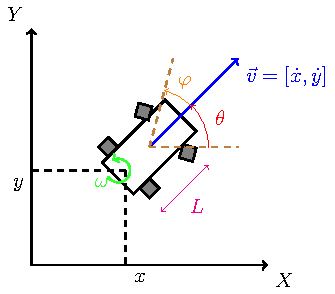
\includegraphics[width=0.5\textwidth]{./Figuras/Carro/Carro}
	\caption{Representación de la posición de un robot móvil con configuración Ackerman.}
	\label{fig:pose}
\end{figure}
\par A saber que el par $(\dot{x}, \dot{y})$ se puede a la vez expresar en términos de $v$ y $\theta$ como $[v\cos(\theta), v\sen(\theta)]$, mientras que el modelo cinemático expresado de manera matricial es el señalado en la Ecuación \eqref{eq:mc}. 
\begin{equation}\label{eq:mc}
	\left[\begin{array}{c}
	\dot{x}\\
	\dot{y}\\
	\dot{\theta}\\
	\dot{\varphi}
	\end{array}\right]=
	\left[\begin{array}{c}
	\cos(\theta)\\
	\sen(\theta)\\
	\frac{\tan(\varphi)}{L}\\
	0
	\end{array}\right]v+
	\left[\begin{array}{c}
	0\\
	0\\
	0\\
	1
	\end{array}\right]\omega
\end{equation}
\par Del robot móvil, las variables a controlar serán su velocidad lineal y su velocidad angular con el vector $u=[v, \omega]^{T}$. En el sistema fijo, el movimiento del robot como bicicleta está sujeto a dos restricciones de movimiento, una para cada rueda, y son el par de ecuaciones que representa la condición de no deslizamiento, Ecuación \eqref{eq:ns}, y la condición de rodamiento puro, Ecuación \eqref{eq:pr}.
\begin{subequations}
	\begin{equation}\label{eq:ns}
		\dot{x}\sen(\theta+\varphi)-\dot{y}\cos(\theta+\varphi)-L\dot{\theta}\cos(\varphi)=0
	\end{equation}
	\begin{equation}\label{eq:pr}
		\dot{x}\sen(\theta)-\dot{y}\cos(\theta)=0
	\end{equation}
\end{subequations}
\subsection{Diseño del controlador}
\label{ssec:dcon}
\par Desde el punto de vista de un conductor humano, la conducción de un vehículo requiere contar con un volante para ajustar la dirección de las ruedas frontales y de un acelerador para regular la velocidad lineal del vehículo. Si se pretende sustituir al conductor humano por una computadora, es necesario entonces establecer un rumbo que permita al controlador manipular la dirección y el acelerador de la manera que lo haría un conductor humano, e incluso mejor. 
\par En la Sección \ref{sec:con} se abordaron los diferentes enfoques de control posibles que se consideraron para este vehículo. Por el trabajo que debe realizar el RMR, la navegación por medio de referencias visuales en el terreno representa una opción para llevar a cabo el control de la plataforma. La navegación de vehículos autónomos se realiza en muchos casos controlando la posición respecto a una trayectoria generada con anterioridad; sin embargo para realizar la planeación de trayectorias y su posterior seguimiento es necesario contar con información previa del entorno sobre el que se navega, y es esta la razón por la que los vehículos autónomos incorporan un sistema GPS para realizar la planeación de la trayectoria con base en el terreno, y de igual manera en los vehículos autónomos a escala que se consultaron en el \autoref{cap:eda} se emula el sistema GPS con una cámara que apunta a un mapa ubicado en el techo del recinto donde se encuentra la pista. Por los alcances propuestos para el proyecto no se cuenta con sistema GPS ni su equivalente para vehículos a escala, con lo cual resulta de mayor conveniencia realizar la navegación reactiva basada en la identificación de elementos en el ambiente; lo que implica mantener al vehículo en el carril por el que se desplaza, además de realizar la identificación de los señalamientos de tránsito.
\par Continuando con la alusión al \autoref{cap:eda}, los proyectos que encabezan las investigaciones de la conducción autónoma suelen emplear metodologías basadas en controladores no lineales, tema que no se abordará en este trabajo. En el flujo de las tareas del vehículo, una vez que las imágenes son obtenidas por la cámara, la identificación de las líneas que limitan al carril es el primer paso del control, a partir de lo cual el error de orientación es la realimentación visual dada al sistema de control. Por un lado, una aproximación emplea una red neuronal que pueda decidir sobre la siguiente acción del vehículo, orientando las ruedas y regulando la velocidad; desde otra perspectiva, un controlador basado en lógica difusa permitiría orientar el vehículo a partir de las funciones de pertenencia que intervienen a la entrada del sistema; en la bibliografía se pueden encontrar casos de control lateral basados en los dos enfoques anteriores, sin embargo las arquitecturas de controladores basadas en PID resultan de mayor revelancia por su integración con el {\it visual servoing} que se encuentra en la bibliografía consultada.
\par Se ha tomado un controlador basado en PID para el seguimiento y permanecimiento en el carril. Con este fin es utilizado el modelo cinemático de la bicicleta para simplificar el problema, y a partir de él se definen las variables de error involucradas en el proceso de permanecimiento en el carril. Considerando una trayectoria establecida en el terreno con una curvatura suave, el vehículo deberá realizar un recorrido paralelo a la trayectoria y lo más cercano a ella. Se cuenta con la Figura \ref{fig:lane} en la que se describen las variables involucradas en el {\it controlador lateral} del vehículo, resaltando a $e$ como el error lateral y a $\delta$ como el error de orientación. El objetivo del controlador implica mantener al vehículo de manera paralela a la trayectoria logrando que el error de orientación sea mínimo, mientras que para lograr que el recorrido paralelo a la trayectoria sea cercano a ella se requiere que el error lateral sea también mínimo. Las variables $e$ y $\delta$ se pueden relacionar con las ecuaciones \eqref{eq:eibvs} y \eqref{eq:dibvs} para el caso del control IBVS o con las ecuaciones \eqref{eq:epbvs} y \eqref{eq:dpbvs} para el caso del control PBVS. De manera objetiva, el vehículo extrae características sólo de la imagen sin importar de manera específica la posición de la propia plataforma, por lo que el controlador IBVS resulta conveniente. El vehículo se encontrará viajando a lo largo del carril, y al ser $e$ de orden mínimo será suficiente controlar $\delta$ a través de $\varphi$, que es el viraje de las ruedas delanteras del vehículo.
\begin{figure}[htbp!]
	\centering
	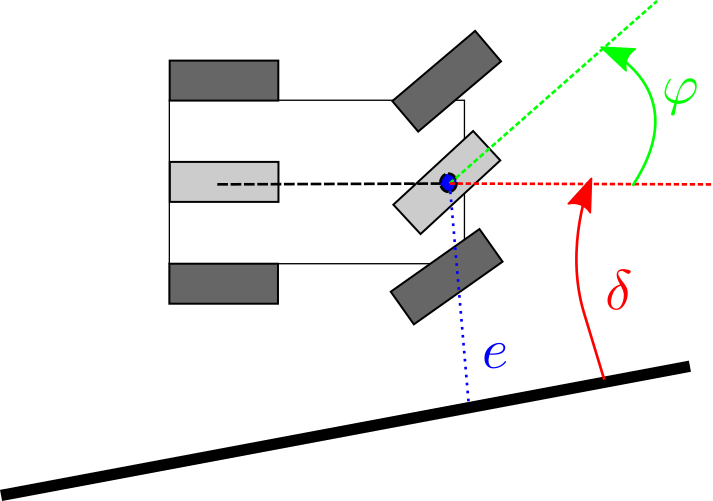
\includegraphics[width=0.5\textwidth]{./Figuras/Lane}
	\caption{Generación del error para un controlador lateral de vehículo autónomo.}
	\label{fig:lane}
\end{figure}
\par Considerando en primer lugar una velocidad constante del vehículo cuando se desplaza sobre el eje $X$ mientras se estabiliza su orientación a través de oscilaciones con amplitud en el eje $Y$; se puede relacionar la distancia recorrida en el eje $X$ con el tiempo transcurrido durante esta acción. Se realizaron una serie de simulaciones aproximando la velocidad del vehículo en la simulación a la del vehículo real (de manera aproximada se ha establecido en *$5.7 \frac{cm}{s}$), tras lo cual se intentaron distintas ganancias $K_{p}$, $K_{d}$ y $K_{i}$ del controlador a modo de proceso de sintonización. Hay que aclarar que el vehículo real contará con valores diferentes en las ganancias en el controlador, ya que las simulaciones no contemplan las perturbaciones producidas por el terreno, como la fricción.
\begin{figure}[htbp!]
	\centering
	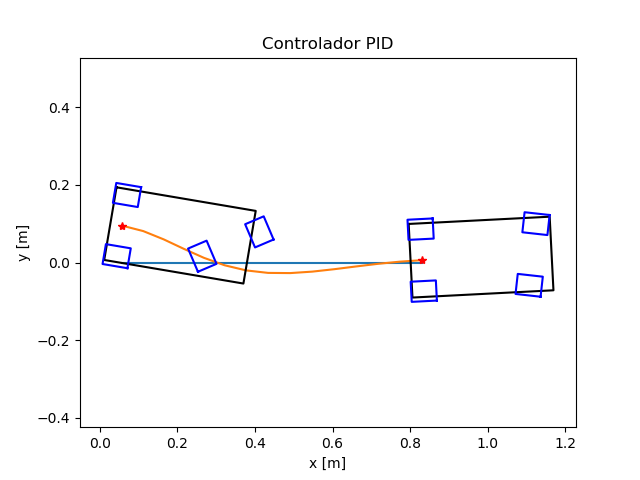
\includegraphics[width=0.7\textwidth]{./Figuras/PIDSim}
	\caption{Simulación del controlador PID.}
	\label{fig:pids}
\end{figure}
\par Se realizaron una serie de simulaciones para sintonizar el controlador de manera inicial. En la Figura \ref{fig:pids} se muestra una de estas simulaciones, en ella se muestra la configuración inicial del robot sobre el plano, además de la configuración final del robot al estabilizarse. En azul se muestra la trayectoria esperada, mientras que en naranja se muestra la trayectoria real. Las ganancias empleadas son *$K_{p}=2.7$, $K_{i}=0.001$ y $K_{d}=5.0$, y aunque el sistema presenta oscilaciones, son de un orden de unos pocos centímetros y no representan un gran problema para la cinemática del vehículo, se establecieron de esta manera para evitar que fueran de mayor magnitud. Los puntos a los que se establece que debe llegar el vehículo están relacionados con la curvatura local del carril, y son obtenidos gracias a la cámara, se toman parámtros importantes de las líneas como su pendiente e intercepto. La simulación que se presenta se realizó en el lenguaje de programación Python, y el listado del código de la misma puede encontrarse en el Anexo \ref{sec:csim}.
\subsubsection{Comportamiento eléctrico}
\label{sssec:elecomp}
\par Existen técnicas de control específicas para motores de CD, sin embargo --y para fortuna-- los carros RC comerciales en su mayoría incorporan un módulo ESC\footnote{Electronic Speed Controller.} que se encarga del control de velocidad del motor CD a través del ancho de pulso que recibe. Es de esta forma que es posible fijar distintos valores de velocidad con distintos anchos de pulso. Este es un funcionamiento similar al de los servomotores de posición. En la Figura \ref{fig:pwm} se muestran algunos de los anchos de pulso principales para un servomotor de posición, donde el estándar bajo el que trabajan involucra una frecuencia base de 50 Hz, logrando así que un servomotor con un pulso de 10 ms alcance una posición de $-90^{o}$, 15 ms equivale a $0^{o}$ y 20 ms equivale a $90^{o}$; en el caso de un motor de CD controlado por un ESC, 10 ms representa la máxima velocidad que alcanza el motor en reversa, 15 ms representa una velocidad cero y 20 ms representa la velocidad máxima que alcanza el motor hacia adelante.
\begin{figure}[htbp!]
	\centering
	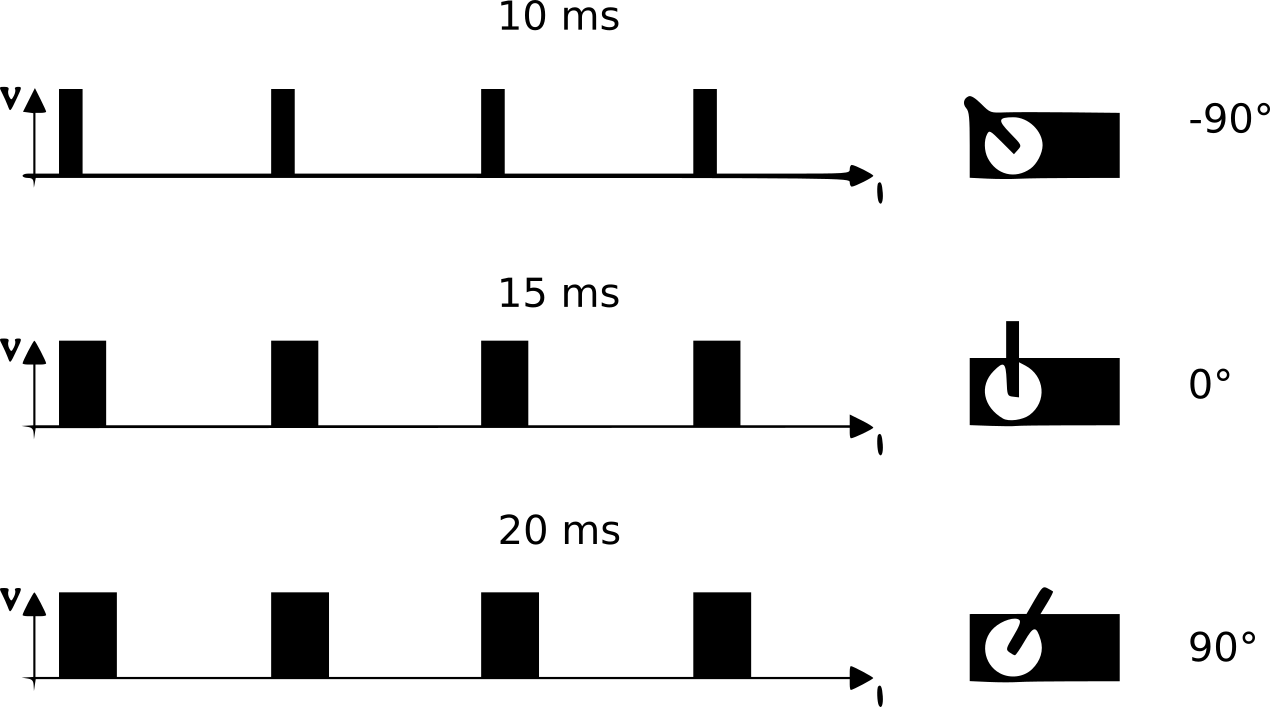
\includegraphics[width=0.5\textwidth]{./Figuras/PWM}
	\caption{Representación de las diferentes señales enviadas a un servomotor.}
	\label{fig:pwm}
\end{figure}
\section{Selección de la plataforma}
\label{sec:selplat}
Dentro de los alcances y objetivos de este proyecto no se encuentran contemplados ni el diseño ni la construcción del chasís del robot, de esta manera es que se vuelve necesario realizar una búsqueda entre los múltiples chasís comerciales, para de esta forma tomar aquellos que se adapten a las necesidades de este Trabajo Terminal. Es habitual que el carro esté ligado a un control remoto que envíe señales para controlar las ruedas de acuerdo a los controles manipulados por el usuario; en este caso se desprecia la teleoperación y en su lugar se controla el vehículo a través de un programa dentro de la computadora embebida, que se encarga de ejecutar los módulos encargados de la interacción con los susbsistemas del vehículo.
\par Dentro de toda la comunidad del modelismo a escala, los vehículos a escala 1:10 son muy populares, y los hay para distintos objetivos. Se pueden encontrar vehículos especializados en velocidades altas y acrobacias sobre terrenos difíciles, los hay también especializados en derrapes y otros sólo de exhibición; además existen clasificaciones generales de acuerdo a su propulsión (existiendo eléctrica con y sin escobillas o de combustión interna).
\par Se tomaron en cuenta las afirmaciones expuestas en la Sección \ref{sec:mc} para eliminar de la selección aquellos vehículos que se encuentren fuera de los propósitos de este proyecto. Por incio de cuentas, como el vehículo se encuentra sobre una superficie plana, entonces no se toman en cuenta los que están diseñados para ir por terrenos accidentados; de acuerdo con la tercera afirmación, no existe deslizamiento entre la rueda y el suelo, por lo que los vehículos diseñados para realizar derrapes no se consideran. Fueron considerados sólo aquellos vehículos de propulsión eléctrica. Como el vehículo opera a velocidades bajas o moderadas sobre un terreno plano, se optó por elegir un vehículo de propósito general. En las tiendas en línea especializadas en vehículos RC se pueden encontrar a los mismos coches en un variado rango de precios, y como no se fija como requerimiento que tenga una alta resistencia a impactos, los chasís metálicos y de fibra de carbono quedan descalificados, y de paso ayuda con la reducción de costos. Es importante mencionar que la búsqueda se realizó dentro de una categoría llamada {\it ready to run} pues estos ya se encuentran preensamblados con un motor de tracción, servomotor de dirección y batería, que a la larga evita hacer múltiples selecciones de componentes.
\par La búsqueda descrita con anterioridad arroja como resultado preferir el modelo VRX-RH1025, cuya imagen se muestra en la Figura \ref{fig:chasis}, en el Anexo \ref{sec:vrx} toman parte los instructivos del ensamble mecánico del carro. Del chasís existen características significativas que a continuación se enumeran:
\begin{itemize}
	\item 364 mm de largo.
	\item 190 mm de ancho.
	\item 285 mm de distancia entre ejes.
	\item Transmisión de 6.5:1.
	\item Ruedas con radio de 65 mm y 26 mm de ancho.
	\item Batería incluida de 7.2 V y 1800 mAh.
\end{itemize}
\begin{figure}[htbp!]
	\centering
	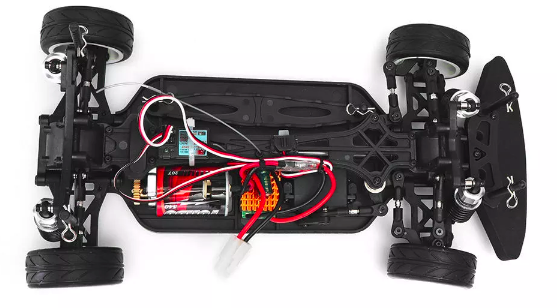
\includegraphics[width=0.7\textwidth]{./Figuras/Chasis}
	\caption{Vista superior del chasís VRX RH1025}
	\label{fig:chasis}
\end{figure}
\par El vehículo cuenta con un módulo ESC modelo H0050B, con el fin de controlar el motor eléctrico con escobillas incorporado, del cual la hoja de datos se puede encontrar en el Anexo \ref{sec:ESC}.
\section{Selección de los componentes electrónicos}
\label{sec:selcomp}
La selección de los componentes electrónicos significa obtener requerimientos de diseño para la Sección \ref{sec:disel}. Los componentes que se seleccionan en esta etapa son la computadora del sistema, el sensor RGB-D y la IMU, al ser los elementos primordiales del sistema, con lo que es posible obtener su consumo eléctrico para la selección de la batería.
\subsection{IMU}
\label{ssec:velor}
Con base en proyectos similares al que aquí se desarrolla, para conocer la velocidad y orientación de vehículo se empleará un módulo de acelerómetro y giroscopio. Existen diferentes módulos que cumplen con esta función, sin embargo aquel que resulta ser de más fácil adquisición es el MPU6050 (Figura \ref{fig:MPU6050}), que involucra seis grados de libertad a través de sus tres ejes para el acelerómetro y otros tres ejes para la rotación con un giroscopio. Este módulo cuenta con una interfaz de comunicación I$^{2}$C, con la cual se transmitirań los datos hacia la computadora.
\begin{figure}[htbp!]
	\centering
	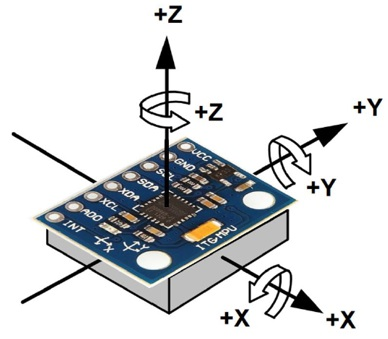
\includegraphics[width=0.35\textwidth]{./Figuras/MPU6050}
	\caption{Módulo de acelerómetro y giroscopio MPU6050}
	\label{fig:MPU6050}
\end{figure}
\par Gracias al uso de este sensor se vuelve posible resolver las restricciones en cuanto a las mediciones obtenidas por el sistema RGB-D. Una brújula provee una orientación absoluta respecto al polo norte magnético, mientras que un giroscopio provee el cambio en la orientación relativa con respecto al cambio en la orientación anterior. Tomando en consideración la sucesión de orientaciones con respecto a una fija e integrando en el tiempo, se puede contar con una orientación absoluta del carro.
\subsection{Sensor RGB-D}
\label{ssec:rgbd}
En realidad son pocos sensores RGB-D en el mercado, y la lista se limita aún más si se consideran sólo los que son compatibles con la librería OpenNI, por lo que es fácil incluir los principales en una tabla para mostrar de manera general sus características y a partir de ello realizar la selección del más adecuado. En la Tabla \ref{tab:rgbd} se consideran los sensores RGB-D principales de cada fabricante, pues dentro de un mismo fabricante se cuentan con características similares, quedan considerados los de características que atiendad a los requerimientos del proyecto.
\begin{table}[htbp!]
	\caption{Sensores RGB-D con sus principales características}
	\label{tab:rgbd}
	\begin{center}
		\begin{tabular}{|p{5cm}|p{7cm}|}
			\hline
			{\bf Cámara} & {\bf Características}\\
			\hline
			Orbbec Astra Pro 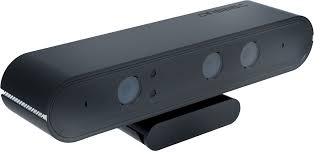
\includegraphics[width=3.5cm]{./Figuras/Orbbec} &
			\begin{compactitem}
				\item 1280x720 pixeles a 30 FPS para RGB.
				\item 640x480 pixeles a 30 FPS para la profundidad.
				\item Rango de operación entre 0.6m y 8m.
				\item FOV de 60$^{O}$ en horizontal, 49.5$^{O}$ en vertical y 73$^{O}$ en diagonal.
			\end{compactitem}\\
			\hline
			Asus Xtion Pro 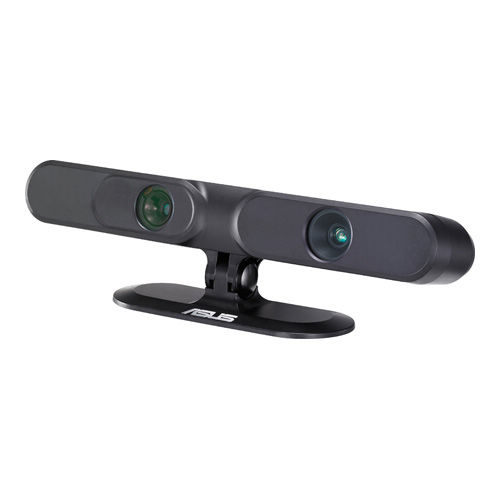
\includegraphics[width=3.5cm]{./Figuras/Asus} &
			\begin{compactitem}
				\item 1280x1024 pixeles a 30 FPS para RGB.
				\item 640x480 pixeles a 30 FPS para la profundidad.
				\item Rango de operación entre 0.8m y 3.5m.
				\item FOV de 58$^{O}$ en horizontal, 45$^{O}$ en vertical y 70$^{O}$ en diagonal.
			\end{compactitem}\\
			\hline
			Intel Realsense SR300 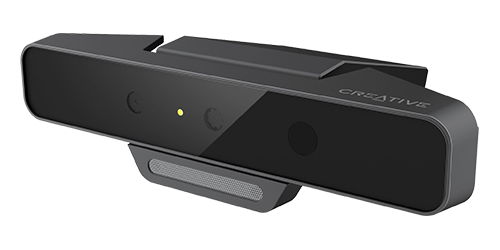
\includegraphics[width=3.5cm]{./Figuras/Intel} &
			\begin{compactitem}
				\item 1920x1080 pixeles a 30 FPS para RGB.
				\item 1280x720 pixeles a 30 FPS para la profundidad.
				\item Rango de operación entre 0.2m y 1.5m.
				\item FOV de 69.4$^{O}$ en horizontal, 42.5$^{O}$ en vertical y 77$^{O}$ en diagonal.
			\end{compactitem}\\
			\hline
		\end{tabular}
	\end{center}
\end{table} 
\par La Tabla \ref{tab:rgbd} muestra los sensores RGB-D de los fabricantes Orbbec, Asus e Intel; para este proyecto no se consideró el Kinect de Microsoft debido a que el mismo se encuentra limitado en sus prestaciones de software y hardware al no contar con conexión USB. Para la selección de la cámara, la característica principal en la que se prestó atención es el rango de operación. El rango de operación determina la distancia mínima a la cual el sensor de profundidad garantiza encontrar puntos de interés, por lo que se requiere contar con un rango en el que el límite inferior sea cercano a la cámara, con lo cual el vehículo podrá operar en una pista también reducida. El límite superior del rango de operación no representa en este caso un parámetro determinante, ya que se trabajará con objetos próximos.
\par Con base en la búsqueda de la cámara con el límite inferior del rango de operación más reducido, se concluyó que las cámaras de la familia {\it Intel Realsense} son las que brindan un rango de operación inferior menor, con 0.2 m. El modelo SR300 de esa familia es el modelo más económico, y de mayor disponibilidad en los tiempos utilizables para este proyecto. El resto de las características técnicas son similares entre los diferentes fabricantes, además de que, aunque la cámara opere con una resolución de 1920x1080 pixeles o 1280x1024 pixeles, se reducirá la resolución de las imágenes para facilitar a la computadora realizar el procesamiento de los datos obtenidos, y el número de imágenes capturadas cada segundo se reducirá de acuerdo a la velocidad con la que navegue el RMR. En este mismo sentido, el FOV\footnote{Siglas en inglés para Campo de Visión} no difiere demasiado entre los tres modelos, y este parámetro no afecta en gran medida la operación del robot.
\par Una ventaja que se obtiene al seleccionar la cámara {\it Intel Realsense SR300} es que el propio fabricante Intel proporciona una SDK\footnote{Software Development Kit} para el manejo de las funciones primarias de la cámara, y ahora es posible la integración con la librería OpenCV. La cámara OpenCV requiere un puerto USB 3.0 para su operación, lo que se añade a los datos que se tomarán en cuenta para la selección de la computadora.
\subsection{Computadora de Placa Reducida}
\label{ssec:comp}
La labor de la computadora a bordo es procesar el volumen de datos que ha sido obtenido por el sensor RGB-D y la IMU. Basándose en los datos que aportan los sensores presentes es que se vuelve posible controlar la velocidad y orientación del vehículo. A partir de la versión 3.4 de la librería OpenCV es necesario contar con 1 Gb de memoria RAM para su instalación cuando se compila desde el código fuente (como en este caso que es necesario enlazar la librería OpenCV con las librerías LibRealSense y OpenNI); y en realidad para la operación posterior esta capacidad mínima depende de las operaciones a realizar, debido a que existen algoritmos bastante rápidos y otros que requieren emplear un mayor poder computacional. Con esto en mente se pre-seleccionaron las siguientes opciones debido a que cumplen con este requisito mínimo.
\par La Raspberry Pi en el modelo 3B cuenta con 1 Gb de memoria RAM, lo cual cumple con este requisito. Buscando contar con una mayor capacidad, se encontró en internet a las computadoras Odroid-XU4 y la Rock64, que representan fuertes candidaturas como computadora del vehículo. Se encontró que la computadora Odroid-XU4 no se encuentra disponible en la tienda oficial y no hay fecha para un relanzamiento; por otro lado en la tienda en línea de la computadora Rock64 se anuncia un nuevo lote disponible a la venta. La Tabla \ref{tab:computadoras} muestra las características de estas tres computadoras a manera de comparación.
\begin{table}[htbp!]
	\caption{Computadoras con sus principales características}
	\label{tab:computadoras}
	\begin{center}
		\begin{tabular}{|p{5cm}|p{7cm}|}
			\hline
			{\bf Computadora} & {\bf Características}\\
			\hline
			Raspberry Pi 3B 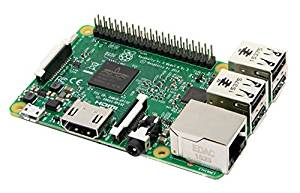
\includegraphics[width=3.5cm]{./Figuras/RPi} &
			\begin{compactitem}
				\item Procesador ARM-8 con 1.2 GHz a 64 bits.
				\item 1 Gb de RAM.
				\item Funciona con memoria micro SD.
				\item Cuenta con conexión USB, Ethernet, WiFi, Bluetooth y GPIO.
				\item Consume 800mA a 5V
				\item Ya se cuenta con ella.
			\end{compactitem}\\
			\hline
			Odroid-XU4 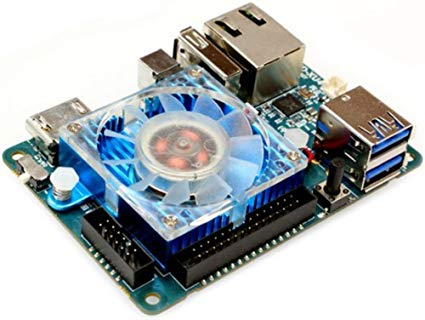
\includegraphics[width=3.5cm]{./Figuras/Odroid} &
			\begin{compactitem}
				\item Procesador ARM-A7 con 2 GHz a 64 bits.
				\item 2 Gb de RAM.
				\item Funciona con memoria micro SD o eMMc.
				\item Cuenta con conexión USB, Ethernet y GPIO.
				\item Consume 4A a 5V.
			\end{compactitem}\\
			\hline
			Pine64-Rock64 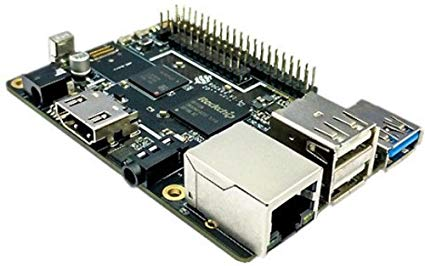
\includegraphics[width=3.5cm]{./Figuras/Rock64} &
			\begin{compactitem}
				\item Procesador Rockchip RK3328.
				\item 4 Gb de RAM.
				\item Funciona con memoria micro SD o eMMc.
				\item Cuenta con conexión USB, Ethernet y GPIO.
				\item Consume 3A a 5V.
			\end{compactitem}\\
			\hline
		\end{tabular}
	\end{center}
\end{table}
\par En el Anexo \ref{sec:pi} se muestran los diagramas para los dos puerto GPIO que incorpora la tarjeta Rock64, que incluyen interfaces de entradas y salidas generales, además de comunicaciones UART, SPI e I$^{2}$C. Los otros periféricos disponibles y de utilidad son los siguientes:
\begin{itemize}
	\item Puerto Ethernet (1).
	\item Puerto USB 2.0 (2).
	\item Puerto USB 3.0 (1).
	\item Jack de audio 3.5 mm (1).
	\item Puerto HDMI (1).
	\item Puerto IR (1).
\end{itemize}
\subsection{Suministro de energía}
\label{ssec:ener}
Se cuenta con dos fuentes de energía separadas. El vehículo ya incluye una batería de 7.2 V a 1800 mAh, la cual le brinda al vehículo una autonomía de 25 minutos aproximadamente en el control de sus motores. Sin embargo para alimentar a la computadora (que a su vez alimentará vía USB a la cámara y vía GPIO a la IMU y a la tarjeta controladora de los motores) se requerirá una fuente de energía separada que brinde al menos la misma autonomía para la computadora.
\begin{figure}[htbp!]
	\centering
	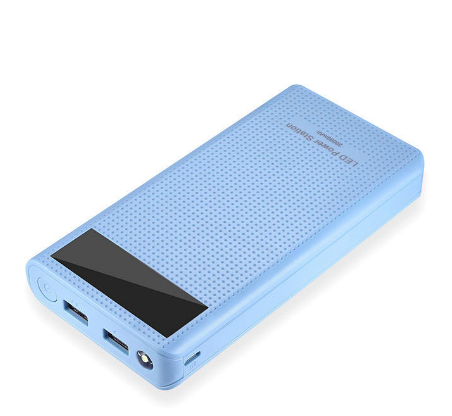
\includegraphics[width=0.4\textwidth]{./Figuras/Power}
	\caption{Batería elegida para el sistema.}
	\label{fig:power}
\end{figure}
\par En la actualidad se cuenta con una amplia variedad de fuentes de energía portátiles, en especial resaltan aquellas empleadas como baterías externas para celulares y tabletas, que son también llamadas {\it powerbank}. Las baterías de las que se habla han adquirido altas prestaciones, con lo que pueden brindar hasta 3.1 A de corriente en algunos casos a través de un puerto USB.
\par Mediante una búsqueda realizada por internet se encontraron diferentes batería portátiles, de las cuales son útiles aquellas que puedan proveer 3.1 A y al menos los 25 minutos de autonomía, del carro. Con una capacidad de 3000 mAh se puede mantener la computadora encendida por una hora antes de recargar la batería, y esta característica resulta suficiente para una sesión de pruebas con el vehículo. La batería elegida suministra la corriente requerida y cuenta con una capacidad de 20000 mAh, suficiente para más de *seis horas de actividad de la computadora y la cámara.
\section{Diseño electrónico}
\label{sec:disel}
En esta Sección se detallan las decisiones de diseño que se tomaron a partir de los elementos más importantes de la selección de componentes: Chasís, sensor RGB-D, computadora, IMU y {\it powerbank}.
\subsection{Interfaz para el control de los motores}
\label{ssec:motcont}
Como ya se ha mencionado antes, para realizar el control de los motores será menester emplear dos señales de PWM; una para el ESC del motor de tracción y otra para el servomotor. Realizar esta acción desde la computadora se vuelve complicado, y esta es una razón suficiente para optar por el diseño de una tarjeta externa basada en microcontrolador como sistema esclavo, que facilite el objetivo de enviar ambas señales de PWM; se propone codificar las características de estas señales PWM para ser enviadas por la computadora mediante comunicación UART.
\par El microcontrolador ATMEGA328P se vende a un precio bajo en comparación de sus prestaciones (de las que sólo por enumerar se cuenta con funcionalidad para comunicación UART, SPI e I$^{2}$C, entradas y salidas generales, ADC, comparadores analógicos, timers de 8 y 16 bits y puertos con salida PWM), lo que lo hace viable para ser el cerebro de la tarjeta que se encargará de controlar los motores. El exceso de puertos de entrada y salida permitirá la escalabilidad del proyecto en un futuro.
\par El diseño de la PCB se realizó en el software Eagle de Autodesk. Lo que se verá a continuación son el esquemático, la vista de las pistas y la vista tridimensional de la PCB en las Figuras \ref{fig:Esque}, \ref{fig:BRD} y \ref{fig:PCB}. El circuito cuenta con un cristal externo para estabilizar la señal de reloj, además el programa que se grabó en el microcontrolador y que controla los motores es el mostrado en el Anexo \ref{sec:micro}.
\begin{figure}[htbp!]
	\centering
	\begin{subfigure}[htbp!]{0.4\textwidth}
		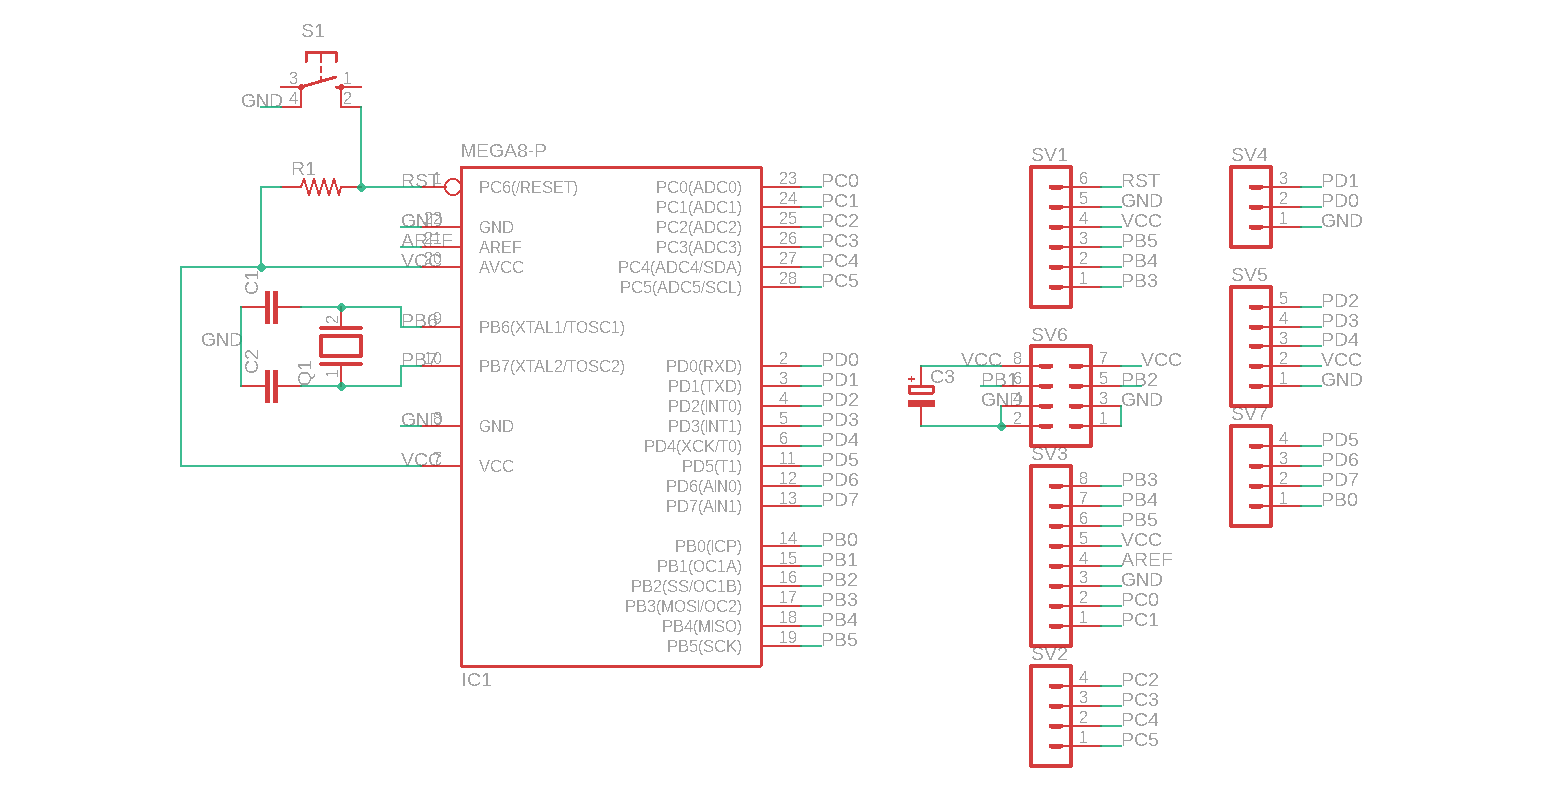
\includegraphics[width=\textwidth]{./Figuras/Esque}
		\caption{Circuito esquemático con las conexiones de la tarjeta.}
		\label{fig:Esque}
	\end{subfigure}
	\begin{subfigure}[htbp!]{0.25\textwidth}
		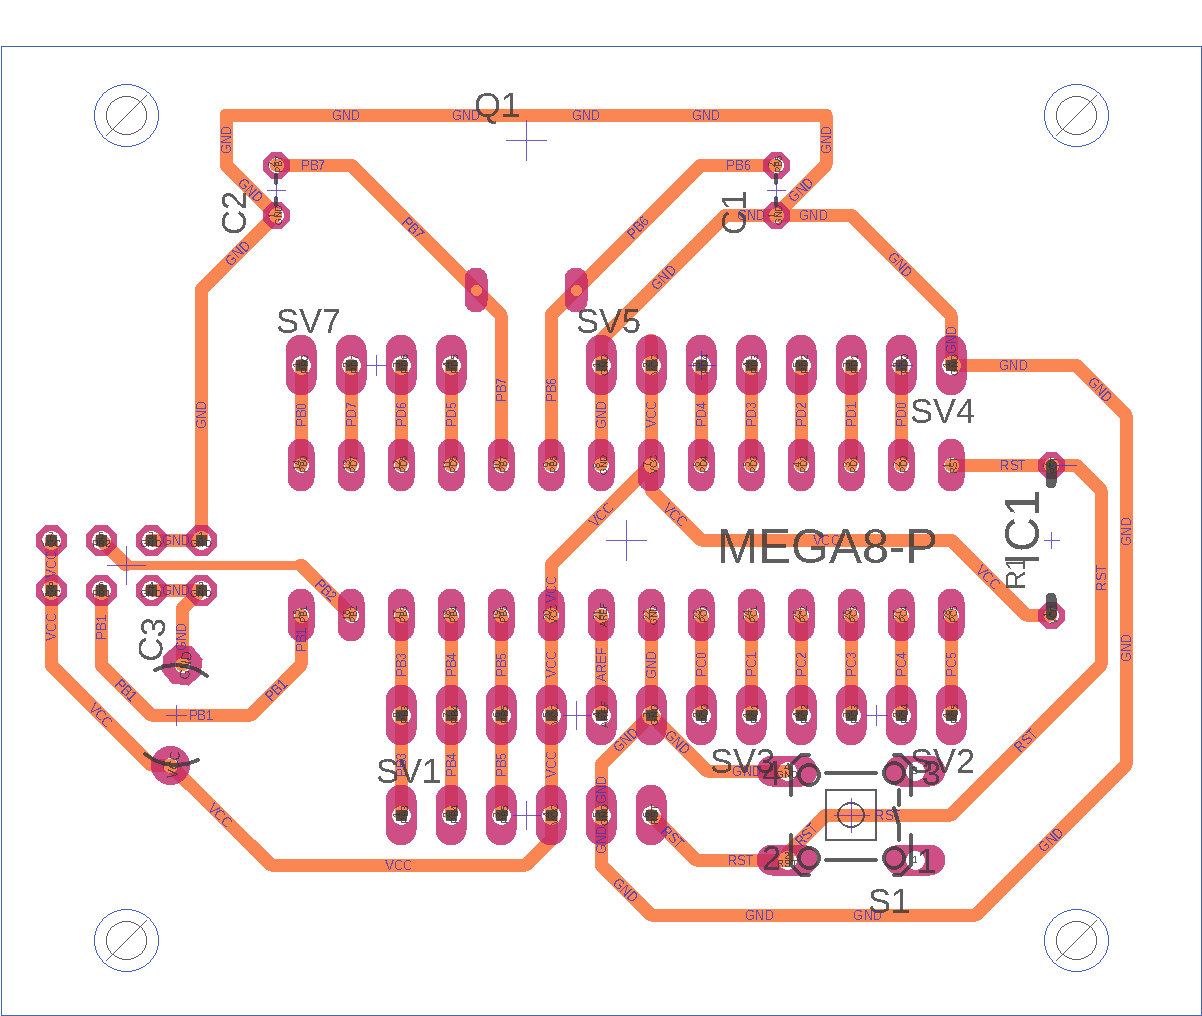
\includegraphics[width=\textwidth]{./Figuras/BRD}
		\caption{Pistas y conexiones del circuito impreso.}
		\label{fig:BRD}
	\end{subfigure}
	\begin{subfigure}[htbp!]{0.3\textwidth}
		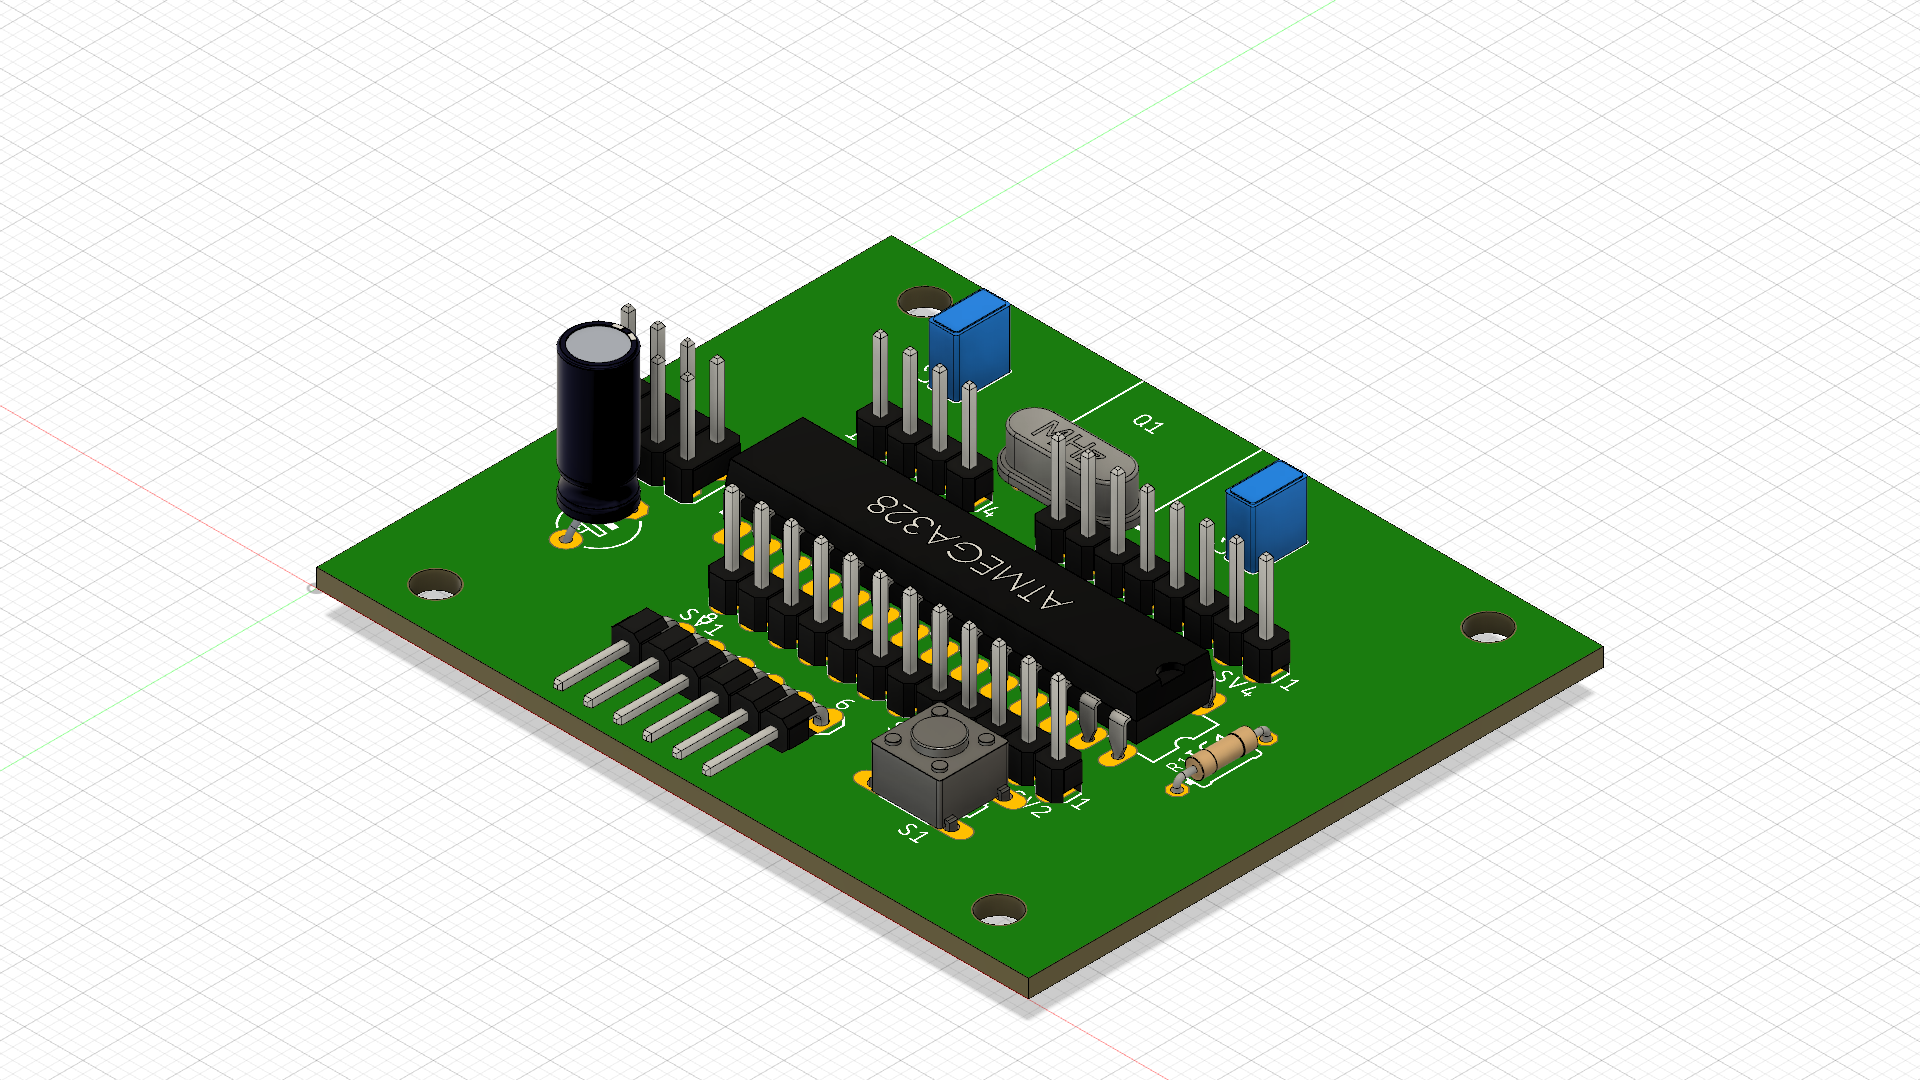
\includegraphics[width=\textwidth]{./Figuras/PCB}
		\caption{Vista tridimensional de la PCB.}
		\label{fig:PCB}
	\end{subfigure}
	\caption{PCB para el control de los motores.}
\end{figure}
\subsection{Conexiones internas}
\label{ssec:conint}
El vehículo funciona de manera inalámbrica sin intervención del operador, sin embargo para este trabajo se implementa una interfaz de comunicación SSH entre la computadora Rock64 y la computadora del usuario para apreciar el procesamiento realizado por la computadora, esto sólo con fines ilustrativos. Para el vehículo es necesario realizar la interconexión de los diferentes módulos que conforman el sistema. El nodo central del sistema es la computadora Rock64, la cual se conecta por medio de un puerto USB 3.0 a la cámara Intel Realsense SR300, y por UART envía de manera codificada los anchos de pulso para el controlador de los motores, que maneja por PWM el ángulo del servomotor de dirección, mientras que también por PWM se maneja la velocidad y la dirección a la que debe girar el motor de tracción. La comunicación con la IMU se da a a través del microcontrolador mediante I$^{2}$C y se comunica la información a la computadora mediante UART. Se creó el diagrama de la Figura \ref{fig:conexiones} para ilustrar las manera en que interactuan las partes del sistema.
\begin{figure}[htbp!]
	\centering
	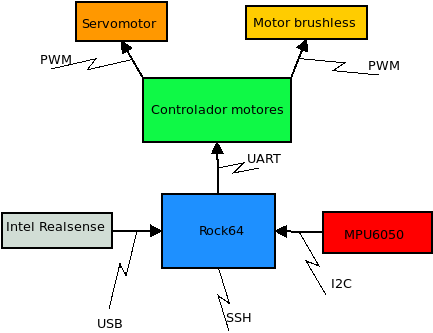
\includegraphics[width=0.5\textwidth]{./Figuras/Conexiones}
	\caption{Diagrama de conexiones internas del vehículo.}
	\label{fig:conexiones}
\end{figure}
\section{Diseño y construcción de la pista de pruebas}
\label{sec:platpru}
El vehículo seleccionado tiene 364 mm de largo y 190 mm de ancho. Otro dato que es importante de conocer son los límites de giro de las ruedas, estando ese rango en el vehículo entre -45$^o$ y 45$^o$. Con base en estos datos se pueden establecer los parámetros con los que debe cumplir la pista de pruebas. Las láminas de MDF de 3 mm de ancho tienen dimensiones de 1.22x2.44 m, con lo que las dimensiones finales de la pista serán múltiplos de 1.22 m.
\par Ya se ha mencionado desde la Sección \ref{ssec:mc} que el radio de curvatura para un vehículo Ackerman puede ser calculado por la expresión $R=L/\tan(\varPsi)$; se ha determinado de manera experimental que el ángulo de giro del vehículo se encuentra entre -45$^{o}$ y 45$^{o}$, de modo que al sustituir la distancia entre ejes y el ángulo de giro máximo se obtiene que el radio de giro para este vehículo en específico es $R=285mm/\tan(45^o)=285mm$, lo que indica que para dar una vuelta perpendicular el vehículo debe empezar a virar antes de que su borde frontal se encuentre en el borde más cercano del camino, de lo contrario se puede salir de la pista.
\begin{figure}[htbp!]
	\centering
	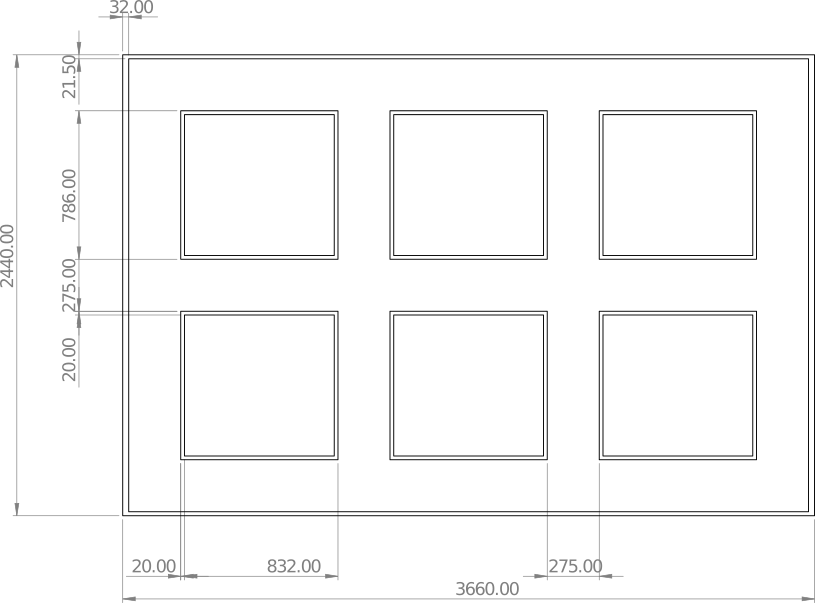
\includegraphics[width=0.8\textwidth]{./Figuras/Pista}
	\caption{Pista de pruebas propuesta acotada.}
	\label{fig:Pista}
\end{figure}
\par Se estableció desde el Protocolo de Investigación que la pista de pruebas contaría sólo con un carril, esto debido a que sólo se proponen maniobras individuales. Para la pista se considera el ancho del carril como 1.5 veces el ancho del vehículo, en este caso da como resultado 275 mm. En proyectos similares se emplean pistas de al menos 8 veces el largo del vehículo para realizar las pruebas. Con lo que se obtiene como resultado 2912 mm, y este número se redondeó para que el resultado encaje con las medidas de las láminas de MDF. Ahora, considerando el boceto de la pista que se propuso en la Figura \ref{fig:PPruebas}, se propone el siguiente croquis de la pista de pruebas. La pista mostrada en el boceto permite la circulación continua del vehículo, una clara ventaja con respecto a lo propuesto en el protocolo de investigación.
\begin{figure}[htbp!]
	\centering
	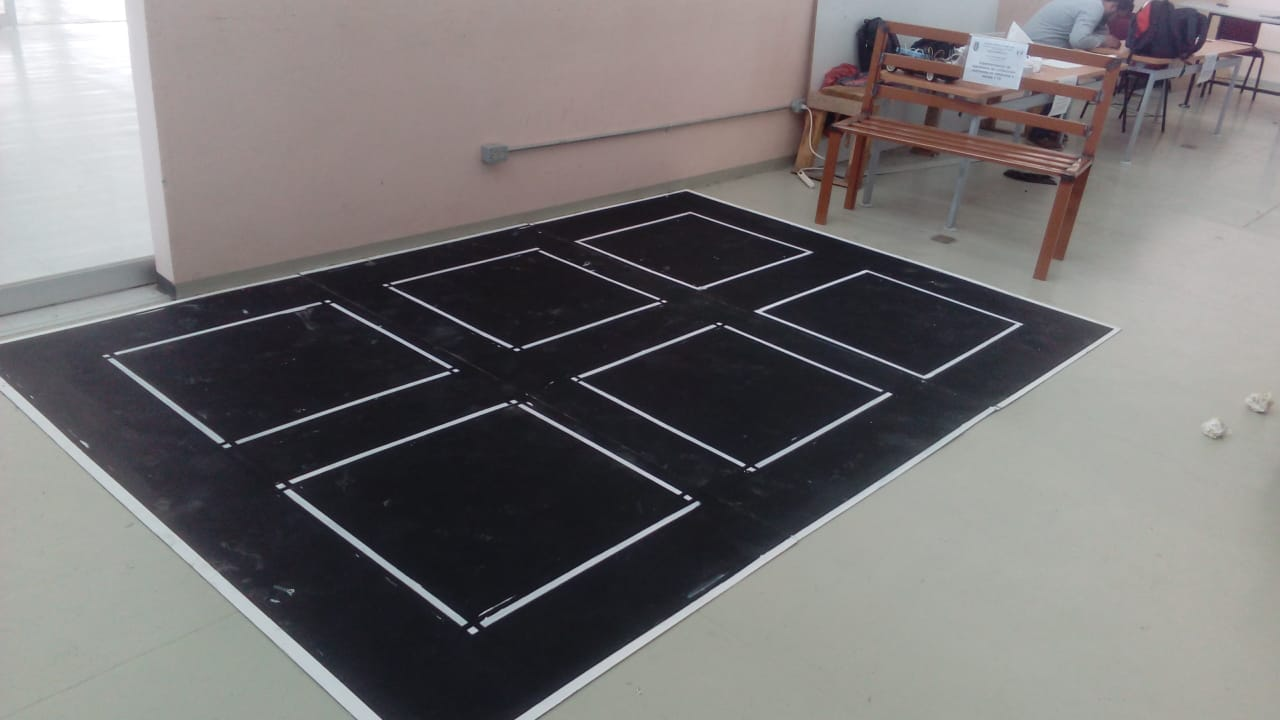
\includegraphics[width=0.8\textwidth]{./Figuras/PistaC}
	\caption{Pista de pruebas construida.}
	\label{fig:pista}
\end{figure}
\par Al inicio de las actividades realizadas para Trabajo Terminal II se encontró la construcción de la pista de pruebas, quedando como resultado la Figura \ref{fig:pista}, que es la unión de los tres tramos de pista.
\begin{figure}[htbp!]
	\centering
	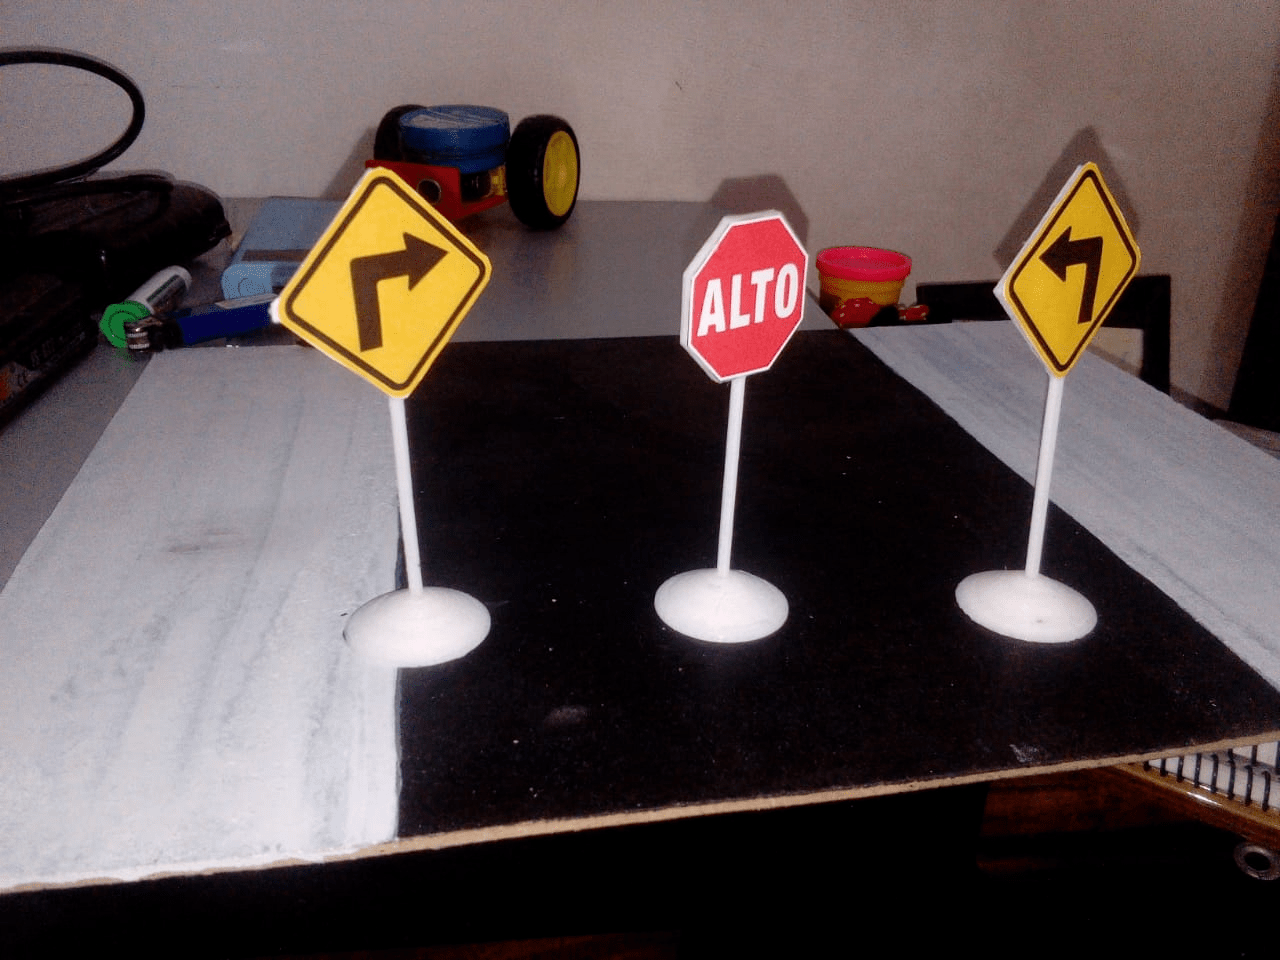
\includegraphics[width=0.5\textwidth]{./Figuras/Senales}
	\caption{Señalamientos fabricados para la pista de pruebas.}
	\label{fig:Sen}
\end{figure}
\par Para la navegación a través del camino por medio de señalamientos el vehículo deberá reconocer las señales de tránsito que se fabricaron en, y que aparecen en la Figura \ref{fig:Sen}. Los señalamientos tienen una altura de 12 cm y están fabricados mediante impresión 3D con PLA. La imagen de la señalética está impresa en papel adherible.
\section{Montaje del vehículo}
\label{sec:monveh}
A continuación se hará una recapitulación de los componentes del vehículo.
\begin{itemize}
	\item {\bf Sensor RGB-D.} Para cumplir con este propósito se seleccionó la cámara Intel Realsense SR300 (Figura \ref{fig:SR300}), la cual cuenta con una resolución de 1920x1080 pixeles en el espacio de color RGB, presenta junto con eso una resolución de 1280x720 pixeles para la profundidad. El rango de operación de la cámara es entre 0.2 y 1.5 m con un campo de visión de 69.4$^o$ en horizontal, 42.5$^o$ en vertical y 77$^o$ en diagonal. A la cámara se le adaptará una zapata que la mantendrá fija al chasís del carro.
	\begin{figure}[htbp!]
		\centering
		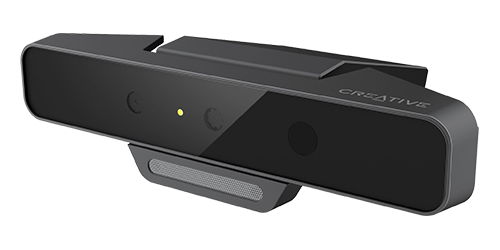
\includegraphics[width=0.4\textwidth]{./Figuras/Intel}
		\caption{Sensor RGB-D Intel Realsense SR300}
		\label{fig:SR300}
	\end{figure}
	\item {\bf Computadora.} La plataforma robótica empleará una computadora Rock64 (Figura \ref{fig:Rock64}) de la compañía Pine64. La computadora Rock64 es una computadora de placa reducida con arquitectura ARM de 64 bits, emplea 4 Gb de memoria RAM, e incorpora un puerto para conectar una memoria microSD y/o eMMC para el almacenamiento. Como periféricos externos, la computadora incorpora dos puertos USB 2.0 y uno 3.0, además cuenta con conector ethernet, jack de audio de 3.5 mm, puerto HDMI, y un conector GPIO Pi-2 y Pi-5. Un elemento que será importante durante las pruebas e implementación de la navegación es el receptor IR incorporado. La computadora se alimenta a 5 V y 3 A mediante un conector de barril de 3.5 mm. El principal sistema operativo soportado por la computadora es el Ubuntu 18.04, sobre el cual se instalará la librería OpenCV y el Realsense SDK de Intel, que serán las encargadas de tomar los datos procedentes de la cámara y el posterior procesamiento.
	\begin{figure}[htbp!]
		\centering
		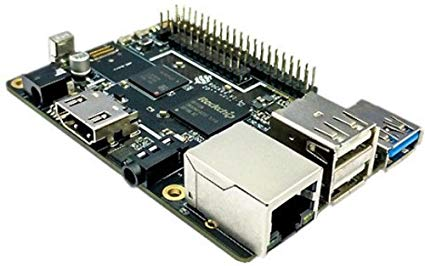
\includegraphics[width=0.4\textwidth]{./Figuras/Rock64}
		\caption{Computador Rock64 de la compañía Pine64}
		\label{fig:Rock64}
	\end{figure} 
	\item {\bf Chasís.} El chasís consiste en dos partes. La parte inferior es el chasís de un vehículo a control remoto a escala 1:10. Para este proyecto se optó por el vehículo VRX RH1025. El chasís superior es una base de acrílico de 3 mm cortada con láser la cual irán montados los demás componentes. El chasís inferior no es un juguete ordinario, pues es una representación realista de un carro real. Cuenta con cuatro ruedas y tracción trasera con una velocidad máxima de 15 km/h. El vehículo cuenta con un motor brushless DC para lograr su desplazamiento, e incluye un circuito ESC para controlarlo usando PWM; además el vehículo cuenta con un servomotor para el control de las ruedas en la estructura Ackerman; y junto con esto una batería de 7.2 V y 1800 mAh, proveyendo energía a estos sistemas. Una imagen del chasís inferior se puede encontrar en la Figura \ref{fig:chasis}; los componentes montados sobre el chasís superior se aprecian en la Figura \ref{fig:chas}, mientras que el plano de la placa puede apreciarse en el Anexo \ref{sec:chass}.
	\begin{figure}[htbp!]
		\centering
		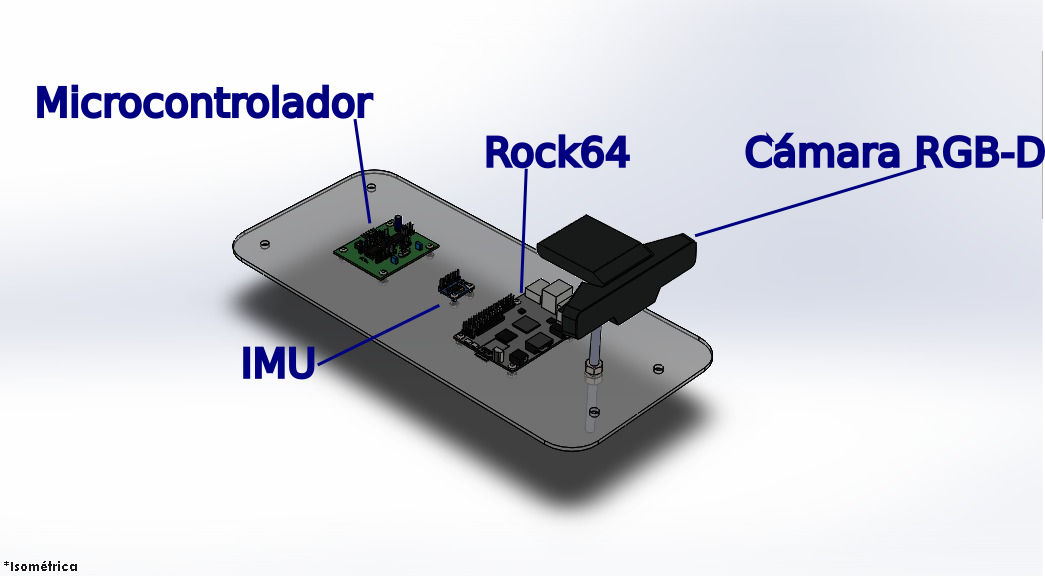
\includegraphics[width=0.8\textwidth]{./Figuras/PlacaEns}
		\caption{Vista superior del chasís superior del vehículo}
		\label{fig:chas}
	\end{figure}
	\item {\bf Acelerómetro y giroscopio.} El módulo de acelerómetro y giroscopio que se tomó en consideración es el MPU6050, el cual cuenta con seis grados de libertad: Tres lineales y tres angulares. El módulo se comunica mediante el protocolo I$^2$C para la transmisión de datos. El módulo de acelerómetro y giroscopio se puede encontrar en la Figura \ref{fig:MPU6050}
	\item {\bf Interfaz para el control de los motores.} Para este propósito se diseñó una tarjeta de circuito impreso con el microcontrolador ATMEGA328P. El objetivo es proveer los puertos para manejar el PWM para el ESC del motor brushless y el servomotor. Los valores necesarios para el manejo de estos anchos de pulso será recibido por el microcontrolador desde la computadora Rock64. Con anterioridad se cuentan cn tres imágenes que muestran más detalle a la PCB, y son las Figuras \ref{fig:Esque}, \ref{fig:BRD} y \ref{fig:PCB}.
	\item {\bf Suministro de energía.} Se mencionó antes que el vehículo a control remoto que fue seleccionado incluye ya una batería que será de uso exclusivo para los motores. Con el objetivo de proveer energía a los sistemas como la computadora y los sensores, se incluye además una batería de que pueda suministrar hasta 3.1 A y 20000 mAh para brindar autonomía durante las pruebas que se realizarán.
\end{itemize}
\par Junto con esto se presenta una tabla con los costos que ha alcanzado el proyecto hasta este momento.
\begin{table}[htbp!]
	\caption{Costos condensados del proyecto.}
	\label{tab:costos}
	\begin{center}
		\begin{tabular}{|c|c|c|c|}
			\hline
			{\bf Componente} & {\bf Modelo} & {\bf Costo} & {\bf Moneda}\\
			\hline
			\hline
			Computadora & Rock64 & \$ 899 & MXN\\
			\hline
			Chasís & VRX RH1025 & \$ 2280 & MXN\\
			\hline
			Cámara & Intel Realsense SR300 & \$ 1780 & MXN\\
			\hline
			Acelerómetro y giroscopio & MPU6050 & \$ 100 & MXN\\
			\hline
			PCB & Control de motores & \$ 100 & MXN\\
			\hline
			Energía & {\it Powerbank} & \$ 399 & MXN\\
			\hline
			Pista & Pista de pruebas & \$ 400 & MXN\\
			\hline
			Extras & Chasís superior y base para cámara & \$ 150 & MXN\\
			\hline
		\end{tabular}
	\end{center}
\end{table}
\par Un proceso de importancia en el proceso fue la puesta a punto de la computadora y la cámara. El proceso involucra la instalación del sistema operativo en la tarjeta microSD, después instalar una larga lista de dependencias de software para culminar con la instalación de las librerías LibRealSense y OpenCV. Se encuentra con más detalle el procedimiento en el Anexo \ref{cap:pap}.
\par En cuanto a lo que concierne de manera general al montaje del vehículo, se inicia con el chasís inferior que está completamente armado de fábrica, y sobre él se coloca la placa que conforma al chasís superior. La placa cuenta con perforaciones para tornillo M3 para montar la computadora, la IMU y la placa controladora de motores. Las conexiones entre los diferentes componentes se realizan con cables Dupont, y se aseguran con cinchos. En las Figuras \ref{fig:fron}, \ref{fig:sup} e \ref{fig:iso} se observan vistas del vehículo ensamblado.
\begin{figure}[htbp!]
	\centering
	\begin{subfigure}[htbp!]{0.4\textwidth}
		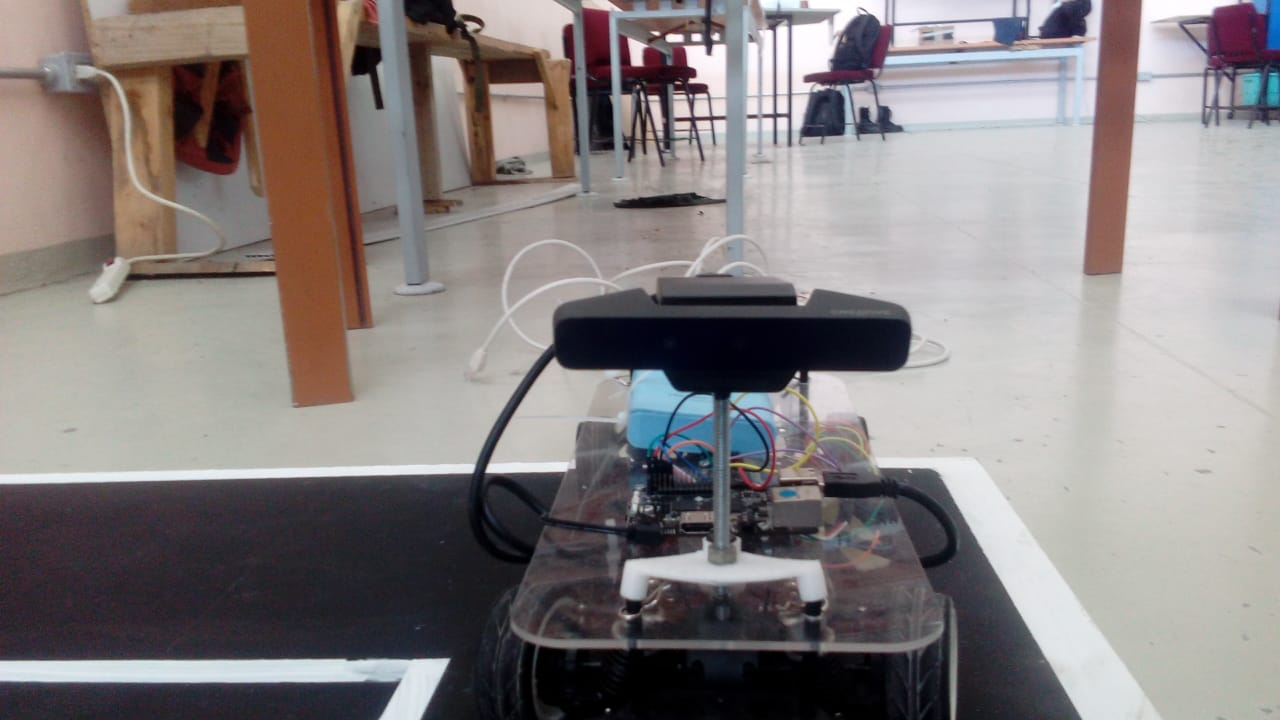
\includegraphics[width=\textwidth]{./Figuras/CarroFron}
		\caption{Vista frontal.}
		\label{fig:fron}
	\end{subfigure}
	\begin{subfigure}[htbp!]{0.4\textwidth}
		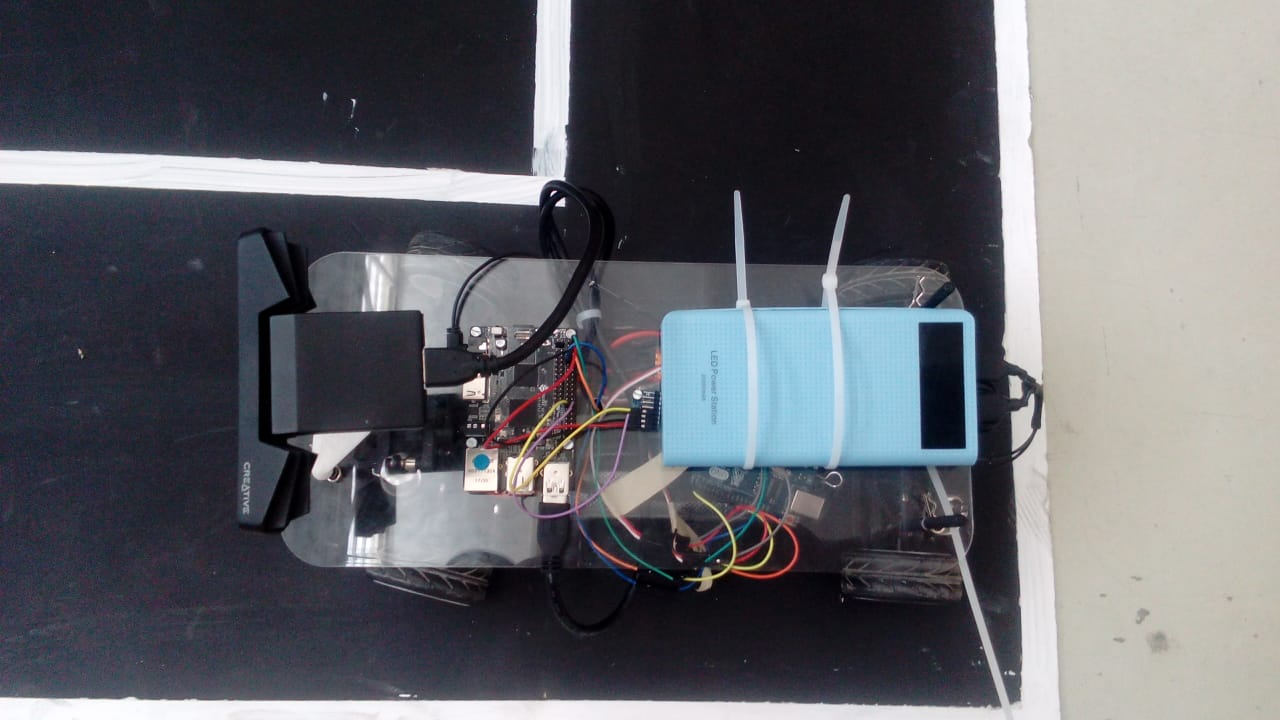
\includegraphics[width=\textwidth]{./Figuras/CarroSup}
		\caption{Vista superior.}
		\label{fig:sup}
	\end{subfigure}
	\begin{subfigure}[htbp!]{0.4\textwidth}
		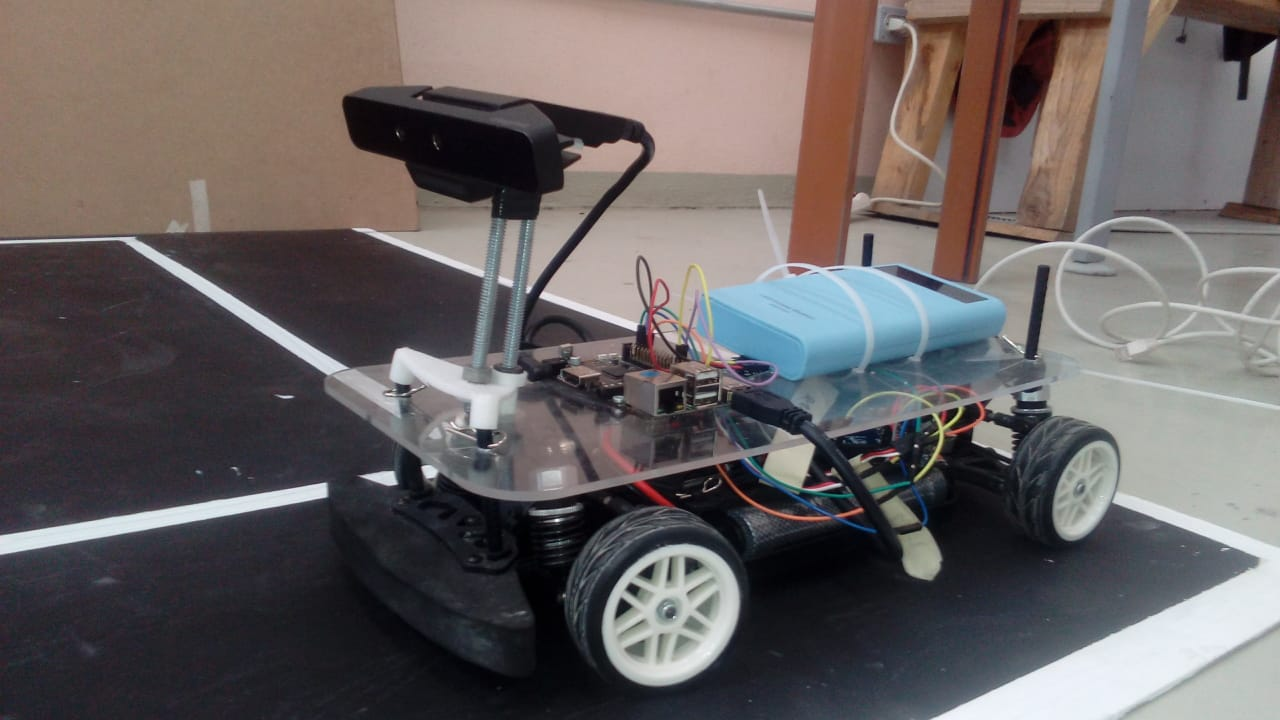
\includegraphics[width=\textwidth]{./Figuras/CarroIso}
		\caption{Vista isométrica.}
		\label{fig:iso}
	\end{subfigure}
	\caption{Diferentes vistas del vehículo armado.}
\end{figure}
\section{Algoritmos e implementación}
\label{sec:alg}
En esta Sección se discute la implementación de los algoritmos de conducción autónoma del vehículo, los cuales se desarrollan en la computadora a bordo. Para la navegación del vehículo se realizó una máquina de estados que en la que se abarca el proceso a partir de una condición inicial de arranque hasta una condición final de paro. Durante el trayecto existirán condiciones intermedias que obligarán a la computadora a tomar una decisión acerca de la acción más conveniente a realizar. Esta primera máquina de estados se muestra en la Figura \ref{fig:me1}.
\par En el diagrama mostrado, el estado {\bf Avanzar} es un nombre abreviado para el mantenimiento en el carril del vehículo, y a partir de ese estado emanan los siguientes. A los estados {\bf Derecha} e {\bf Izquierda} se accede al haber detectado el vehículo la correspondiente señal de tránsito, y vuelven al estado {\bf Avanzar} al momento en el que el vehículo ha concluido la maniobra. El estado {\bf Alto} es el que se obtiene cuando el vehículo se encuentra con un semáforo cuya luz encendida es la roja, y permanece en él hasta que la luz cambie a verde. Por último, el estado {\bf Final} sucede cuando el vehículo se encuentra con una señal de Alto.
\begin{figure}[htbp!]
	\centering
	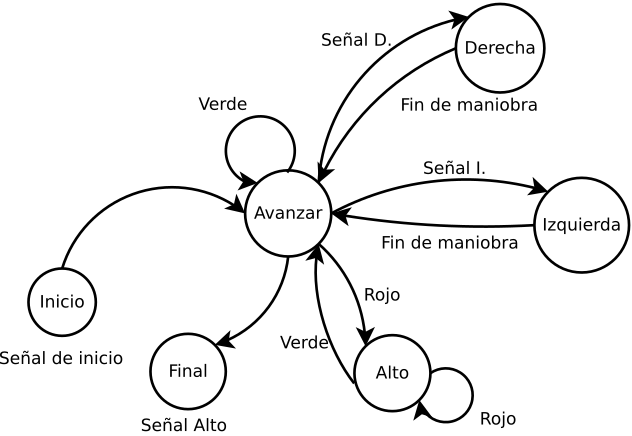
\includegraphics[width=0.7\textwidth]{./Figuras/ME1}
	\caption{Máquina de estados para la navegación del vehículo.}
	\label{fig:me1}
\end{figure}
\par A continuación se desglosa cada una de las actividades en los estados y los propios algoritmos empleados para el mantenimiento en el carril y el reconocimiento de estructuras.
\subsection{Mantenimiento en el carril (Avanzar)}
\label{ssec:ava}
Esta acción se compone de varias etapas, siendo la primera el propio reconocimiento del carril. El reconocimiento del carril sigue la secuencia mostrada en la Figura \ref{fig:pipe}, donde el primer paso consiste en la propia captura de la imagen.
\begin{figure}[htbp!]
	\centering
	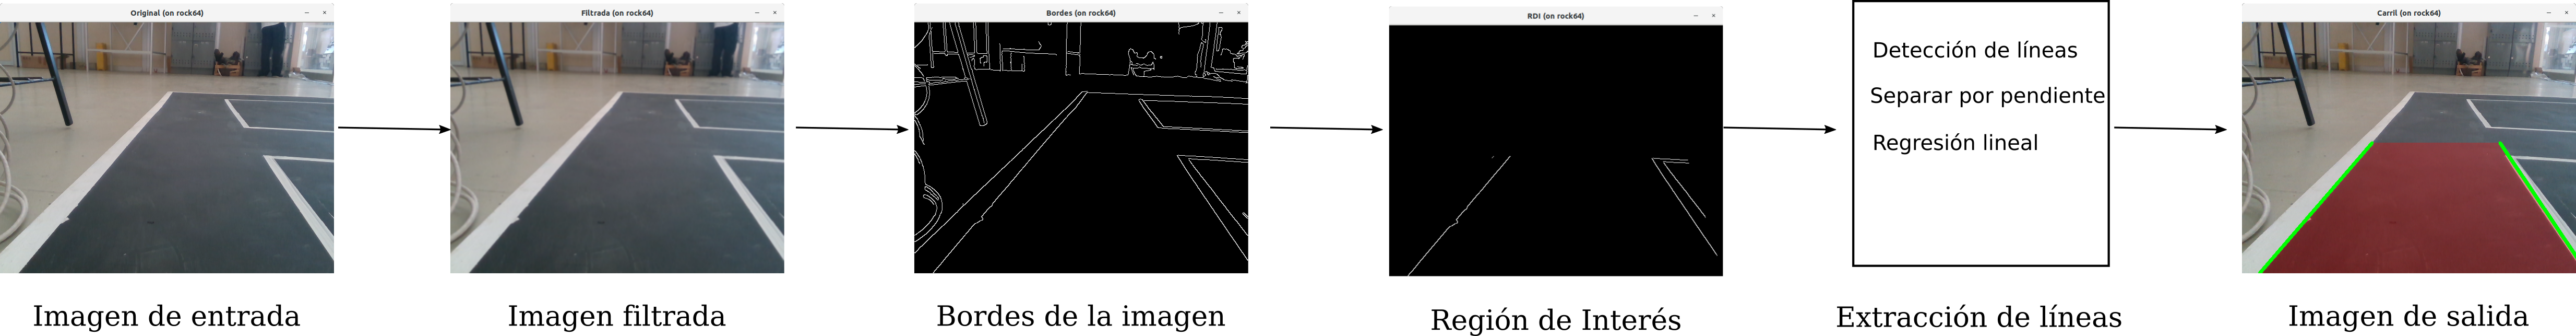
\includegraphics[width=\textwidth]{./Figuras/Pipe}
	\caption{Flujo de trabajo para el reconocimiento del carril}
	\label{fig:pipe}
\end{figure}
\par El proceso que desemboca en la obtención de las características de las líneas que definen los extremos del carril inicia con la imagen de color capturada por la cámara, a la cual se le aplica un filtro a la imagen capturada se le aplica un filtro gaussiano con un núcleo de dimensión (3x3) que reduce el ruido provocado por efectos de iluminación brillo por iluminación. La imagen filtrada pasa por un proceso de resaltamiento de bordes con el operador Canny, en el que la imagen resultante ahora sólo contiene elementos blancos y negros, de los cuales sólo es importante un segmento trapezoidal que contiene únicamente el carril. En la imagen de la región de interés ahora se pueden buscar líneas gracias a la transformada de Hough, sin embargo el número de líneas detectadas es alto, y se requiere  filtrar aquellas que son de importancia; un criterio para realizar la separación es de acuerdo a su pendiente, puesto que las líneas a la izquierda del carril tienen pendiente negativa y las que se encuentran a la derecha tienen pendiente positiva; a ambos lados se almacenan en un vector. Por último, de las características de las líneas a ambos lados se puede realizar una interpolación lineal para ajustar sólo una línea a cada lado del carril, de la que se conoce su pendiente y su intercepto; la imagen mostrada al final de la Figura \ref{fig:pipe} muestra las pendientes a cada lado del carril junto con el área encerrada entre ellas.
\par Como siguiente paso en la preservación del carril, se toman las pendienes de ambas líneas y se suman (una pendiente es positiva y la otra negativa), siendo el resultado la pendiente en la línea que une la intersección de las dos rectas con el centro del inicio de ambas líneas. El controlador toma como entrada esta pendiente y busca llevarla a cero a lo largo de todo el recorrido, como se pantea en la Sección \ref{ssec:dcon}.
\par En las simulaciones se presentaron las ganancias tomadas para el carro, sin embargo para el carro real fue necesario recalcular las ganancias, y el proceso se realizó en tres etapas: primero se hizo teniendo el vehículo estático mientras reconocía el carril, y se llevaron las ganancias del controlador PID hasta que en cada iteración del algoritmo había menos de *0.01 \% de error; la segunda etapa resultó similar, teniendo la diferencia de que ahora el servomotor encargado de la dirección intenta seguir la línea media del carril; la tercera etapa consistió en corregir las oscilaciones mientras que vehículo se encontraba avanzando en un tramo recto de pista a una velocidad constante. Las ganancias obtenidas son: *$K_{p}$, $K_{d}$ y $K_{i}$ 6.5, 10.0 y 0.0001, como corresponde.
\subsection{Reconocimiento de estructuras}
\label{ssec:rde}
Considerando que el sensor RGB-D provee una imagen como:
\begin{itemize}
	\item Una imagen a color en formato RGB.
	\item Un mapa de profundidad con las intensidades que representan distancia.
\end{itemize}
\par Se puede  tomar como referencia el trabajo publicado en \cite{herediafavieriReconocimientoObjetosImagenes2015}, en el que se cuenta con algoritmos para relacionar datos de 2D y de 3D. El sensor RGB-D proporciona un cuadro con más de 300, 000 puntos. Tal y como ocurre en la mayoría de las aplicaciones de la robótica móvil, se puede simplificar el proceso si el robot se considera plano y su forma viene determinada por el mayor polígono que circunscribe las distintas secciones en altura de éste. Una solución eficiente y que no compromete la eficacia del algoritmo reactivo  utilizado consiste en reducir la información 3D obtenida y proyectarla sobre el plano 2D en el que se encuentra el robot. La simplificación resultante consiste en un barrido horizontal que contiene las mediciones más cercanas a los obstáculos presentes a diferentes alturas.
\par Puede ser útil segmentar el mapa de profundidad a partir de la información tomada por la imagen a color. La detección de elementos como semáforos y señalamientos de tránsito se puede realizar mediante el emparejamiento de plantillas a partir de imágenes de prueba, con lo que los algoritmos de FAST, SIFT, SURF y otros, resultan útiles para encontrar la región de la imagen donde se encuentra el señalamiento, y encontrar la distancia a él gracias al mapa de color.
\par El subsecuente proceso para la conversión de datos involucra asumir que se cuenta ya con una imagen a color y un mapa de profundidad provistos por la cámara; el proceso se basa en el algoritmo SURF, a partir de lo cual se sigue el siguiente procedimiento de la manera siguiente:
\begin{itemize}
	\item Detectar características en la imagen objeto (este procedimiento se realiza para cada señal).
	\item Detectar características en la imagen objeto (este procedimiento se realiza para cada cuadro).
	\item Emparejar las características entre ambas imágenes y se calcula el valor de correlación.
	\item Si el nivel de correlación es mayor a 0.80, se obtiene el centro de la imagen, se calcula la profundidad en ese punto y se dibuja en la imagen el área que delimita a la señal en la escena. De lo contrario continua buscando correlaciones en la imagen.
\end{itemize}
\begin{figure}[htbp!]
	\centering
	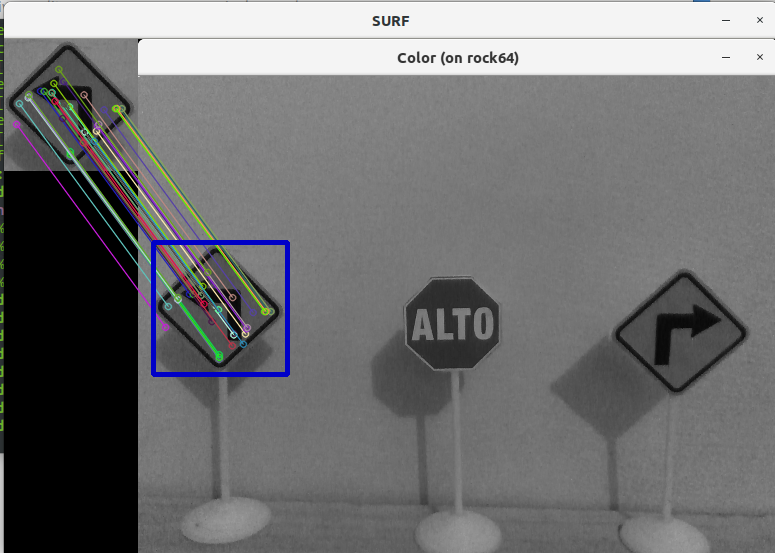
\includegraphics[width=0.3\textwidth]{./Figuras/SURFDere}
	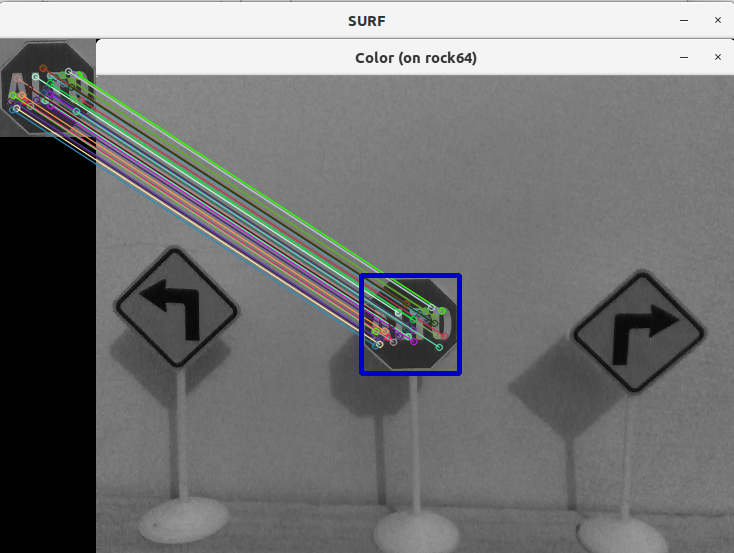
\includegraphics[width=0.3\textwidth]{./Figuras/SURFAlto}
	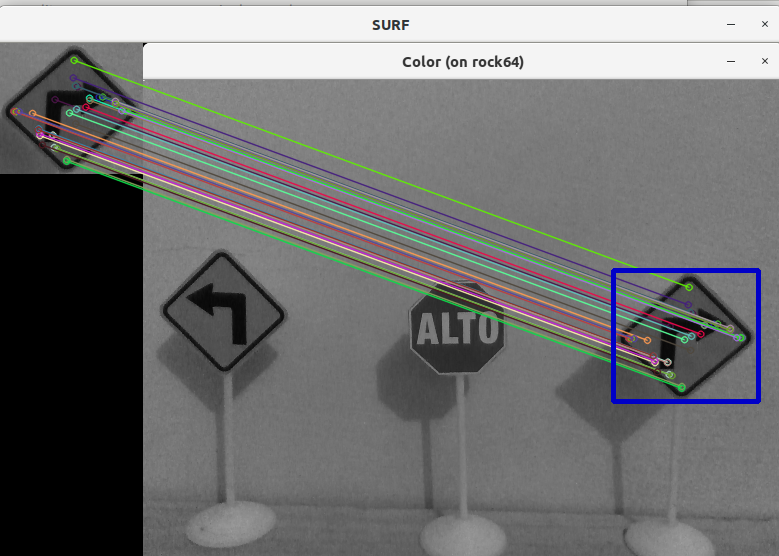
\includegraphics[width=0.3\textwidth]{./Figuras/SURFIzq}
	\label{fig:surf}
	\caption{Aplicación del algoritmo SURF para la detección de señales.}
\end{figure}
\par En las pruebas realizadas se comprobó la eficacia del algoritmo SURF para la detección de los señalamientos de tránsito, las pruebas se encuentran en la Figura 4.19, donde en la esquina superior izquierda se encuentra la imagen objeto, mientras que la imagen escena representa la mayor parte de la imagen. Las líneas de múltiples colores unen los descriptores de ambas imágenes, mientras que el cuadrilátero azul muestra la localización de la imagen objeto dentro de la escena.
\par Para la última parte del procedimiento, que involucra la distancia al objeto, se muestra con la Figura \ref{fig:dist} la distancia al centro de una señal de alto dentro de la imagen de profundidad.
\begin{figure}[htbp!]
	\centering
	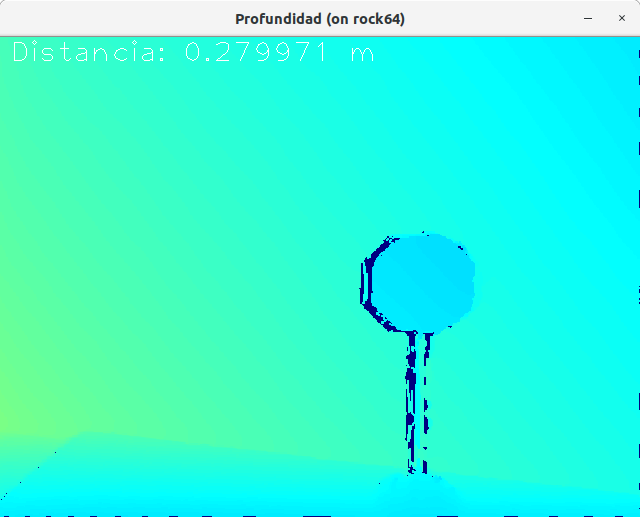
\includegraphics[width=0.5\textwidth]{./Figuras/Distancia}
	\caption{Distancia al señalamiento.}
	\label{fig:dist}
\end{figure}
\par El procedimiento es similar para la detección de semáforos. Una vez que la imagen objeto (semáforo de prueba) se empareja en la imagen de escena, se segmenta la imagen por color de acuerdo al que se busca (Rojo, Verde o Amarillo) y se buscan círculos en la imagen. Un ejemplo del procesamiento se muestra en la Figura \ref{fig:sema}, resaltando la luz roja del semáforo. El dibujo del círculo para señalar la luz se realizó en la imagen segmentada en color con el objetivo de lograr que se aprecie.
\begin{figure}[htbp!]
	\centering
	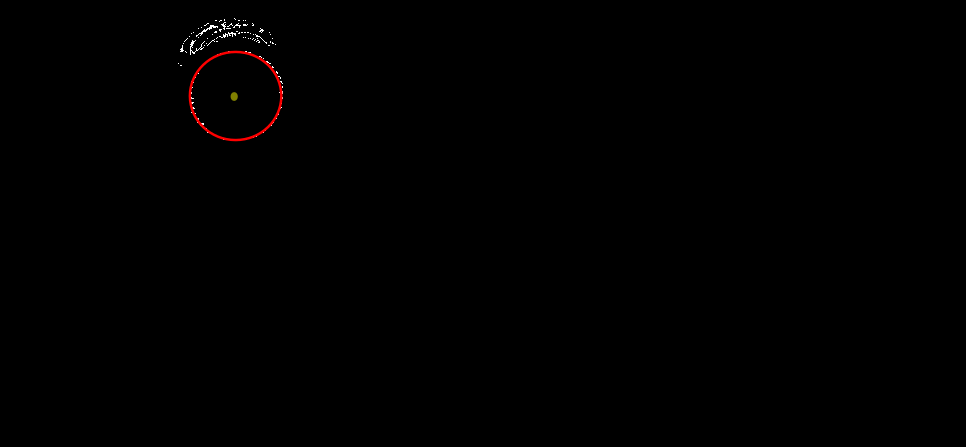
\includegraphics[width=0.5\textwidth]{./Figuras/Sema}
	\caption{Localización de luz roja de un semáforo.}
	\label{fig:sema}
\end{figure}
\subsection{Programación}
Todos los algoritmos que se observan a lo largo de la sección se programaron en C++ usando la librería OpenCV (enlazada con LibRealSense y OpenNI). Se dividió el problema principal en subsistemas, y de cada uno de ellos se construyó una clase compuesta por un archivo de cabecera y uno de funciones. Se cuenta en la Figura \ref{fig:dep} con las dependencias entre cada uno de las componentes de software, teniendo el la parte superior al progama principal y a los archivos de prueba de cada uno de los módulos.
\begin{figure}[htbp!]
	\centering
	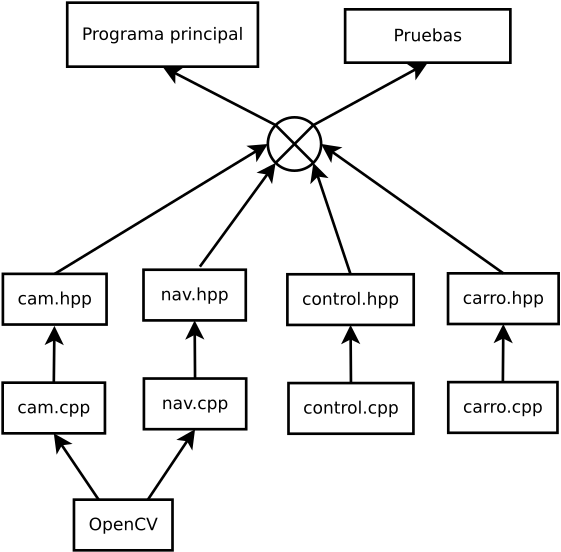
\includegraphics[width=0.5\textwidth]{./Figuras/Dependencias}
	\caption{Diagrama de dependencias de los componentes.}
	\label{fig:dep}
\end{figure}
\par En los Anexos \ref{sec:cam}, \ref{sec:cont}, \ref{sec:car} y \ref{sec:main} se presentan los subsistemas del sistema como clases y además se presenta el programa principal. Se omiten los archivos de prueba de los módulos. Los diagramas UML de las cuatro clases principales del proyecto se presentan en las Figuras \ref{fig:camC}, \ref{fig:controlC} y\ref{fig:carroC}.
\begin{figure}[htbp!]
	\centering
	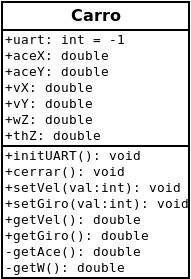
\includegraphics[width=0.3\textwidth]{./Figuras/carroClass}
	\caption{Clase Carro}
	\label{fig:carroC}
\end{figure}
\par La Clase Carro involucra las variables obtenidas por la IMU, y también trabaja con el UART del microcontrolador.
\begin{itemize}
	\item {\it initUART}. Inicializa la comunicación UART entre la tarjeta con el microcontrolador.
	\item {\it cerrar}. Termina la comunicación UART.
	\item {\it setVal}. Envía al carro los valores de la velocidad y el ángulo de las ruedas.
\end{itemize}
\begin{figure}[htbp!]
	\centering
	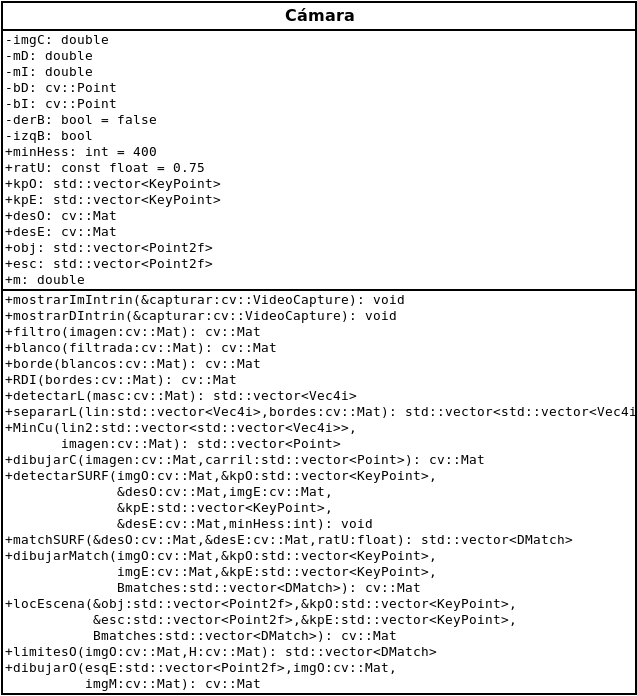
\includegraphics[width=0.7\textwidth]{./Figuras/camClass}
	\caption{Clase Cámara.}
	\label{fig:camC}
\end{figure}
\par La clase maneja la información relacionada al sensor RGB-D.
\begin{itemize}
	\item {\it filtro}. Aplica filtro gaussiano a la imagen de entrada para remover el ruido 
	\item {\it blanco}. Convierte la imagen a HSV para detectar las líneas blancas de la imagen.. 
	\item {\it bordes}. Detecta todos los bordes en la imagen filtrada. 
	\item {\it RDI}. Aplica una máscara poligonal a la imagen para reducir la región de interés. 
	\item {\it detectarL}. Emplea la transformada de Hough probabilística para obtener todos los segmentos de línea en la región de interés.
	\item {\it sperararL}. Separar las líneas a la izquierda y a la derecha del carril 
	\item {\it MinCu}. Se encarga de tomar todas las líneas a ambos lados del carril para interpolar una sola línea a cada lado del carril. 
	\item {\it dibujarC}. Se encarga de mostrar las líneas detectadas para el carril junto con el área encerrada entre ellas. 
	\item {\it detectarDescO}. Se encarga de tomar las imágenes y por medio del algoritmo SURF encontrar los descriptores en la imagen de objeto. 
	\item {\it detectarDescE}. Encuentra los descriptores de la escena. 
	\item {\it match}. Empata los descriptores del objeto con los de la escena. 
	\item {\it dibujarMatch}. Muestra los matches entre el objeto y la escena de manera gráfica. 
	\item {\it locEscena}. Relaciona las transformaciones geométricas entre los descriptores del objeto con los descriptores de la escena. 
	\item {\it limitesO}. Determina los límites del objeto y su correspondencia en la escena. 
	\item {\it dibujarO}. Dibuja al objeto encerrado dentro de la escena. 
	\item {\it Alto}. Condensa los parámetros necesarios para buscar la señal de alto en la escena. 
	\item {\it Izquierda}. Condensa los parámetros necesarios para buscar la señal de vuelta a la izquierda en la escena. 
	\item {\it Derecha}. Condensa los parámetros necesarios para buscar la señal de vuelta a la derecha en la escena.
	\item {\it getDistancia}. Obtiene la distancia del punto p con la información de la imagen de profundidad.
	\item {\it dibujar}. Se encarga de mostrar las líneas detectadas para el carril junto con el área encerrada entre ellas. Muestra los señalamientos encerrados y muestra las distancias al final del camino detectado y a los señalamientos. 
\end{itemize}
\begin{figure}[htbp!]
	\centering
	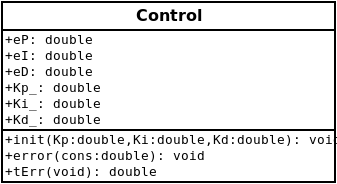
\includegraphics[width=0.6\textwidth]{./Figuras/controlClass}
	\caption{Clase Control}
	\label{fig:controlC}
\end{figure}
\par La clase maneja la información relacionada al controlador PID. El constructor toma los valores deseados de las ganancias $K_{p}$, $K_{I}$ y $K_{D}$.
\begin{itemize}
	\item {\it init}. Inicializa las variables globales de la clase con los valores locales dados.
	\item {\it error}. Actualiza los valores del error en el controlador.
	\item {\it tErr}. Emplea todos los errores y las ganancias para calcular la compensación.
\end{itemize}